%!TEX root = ../template.tex
%%%%%%%%%%%%%%%%%%%%%%%%%%%%%%%%%%%%%%%%%%%%%%%%%%%%%%%%%%%%%%%%%%%
%% chapter1.tex
%% NOVA thesis document file
%%
%% Chapter with introduction
%%%%%%%%%%%%%%%%%%%%%%%%%%%%%%%%%%%%%%%%%%%%%%%%%%%%%%%%%%%%%%%%%%%
\typeout{NT FILE chapter6.tex}%

\chapter{Advanced Feedback}
\label{chap:algo}

Providing meaningful feedback is a complex challenge. In this chapter, we describe how this challenge was addressed. We begin by identifying the key aspects that contribute to producing meaningful feedback. We then present the algorithm developed to tackle the problem, followed by examples that illustrate how feedback can be generated from it. After that, we provide an overview of the algorithm’s implementation, including its testing process and performance results. Finally, we outline future work that can be developed using this algorithm.

\section{Objectives}
Before we introduce the proposed algorithm, we must clarify its main goal. We want our algorithm to be able to support advanced feedback for students learning and practicing the construction of \gls{ND} proofs. Such effective feedback system should be able to deliver relevant information to assist students at any stage of their exercise resolution. Focusing on this main goal, we identified five fundamental objectives a well-designed feedback system should satisfy:

\begin{itemize}

\item \textbf {Context-aware feedback:} The system should be able to adapt to the student's approach, following their reasoning throughout the proof. Since \gls{ND} exercises can often be solved in multiple valid ways, students may choose different strategies or shift directions during resolution. The feedback system must be flexible enough to track their logic and offer guidance aligned with the student's chosen proof strategy, rather than enforcing a single ideal solution.

\item \textbf {Providing guidance on rule applications:} Some rule applications in \gls{ND} are not obvious, making it difficult for students to progress. A paradigmatic example is the case of proofs by contradiction, which is a distinctive feature of classical logic. In some cases no direct proof exists, and the result can only be proved by contradiction: \(\varphi\) is proved by assuming \(\neg \varphi\) and showing that this leads to a contradiction. The feedback system should be able to identify such situations and suggest the appropriate rule applications.

\item \textbf {Breaking proofs into smaller sub-proofs:} Proofs in ND are incrementally built from smaller proofs. Dividing proofs into smaller steps reduces the cognitive load and simplifies reasoning. Therefore, the feedback system should encourage students to start with smaller proofs and incrementally build the main proof. 

\item \textbf{Indicating the distance to a solution:} Showing how many steps (rule applications) are needed to complete the proof helps students maintain focus and gain a clear sense of progress.

\item \textbf{Improvements in the proof:} Providing feedback about irrelevant steps taken or possible shortcuts that could make the proof clearer. It should also allow visualizing different ways to tackle the same problem.

\end{itemize}

Designing an algorithm that provides the basis for a feedback mechanism satisfying the above requirements is quite challenging. We aim to provide structured and clear information, as a tool for helping students to overcome the usual challenges of producing \gls{ND} proofs.

\section{Algorithm}
The algorithm we developed is goal-oriented. Its basic idea is to simplify the original problem into smaller, more manageable sub-problems by applying rules, until it reaches a case that the goal can be directly solved. The proposed algorithm is capable of addressing all the previously stated objectives, and it is applicable to both \gls{PL} and \gls{FOL}. The whole process is structured into three sequential steps discussed in the next sections.

\subsection{Transition Graph}
The first step is to create the so-called \gls{TG}. This graph stores the formulas that might be part of the final proof, as well as the rules that can be applied to each formula.  We can imagine this graph as a data structure that stores all possible "moves" that our "game" can support.

To generate the graph, we need to specify the main goal \(\Gamma \vdash \varphi\), which is the problem itself, and the target goal \(\Sigma \vdash \theta\), which is the part of a student's proof that needs to be completed. The main goal is used to generate all the natural proof paths, which are proofs built using only formulas derived from decomposing the main goal. The target goal, on the other hand, can sometimes be used to generate non-natural proof paths. By this, we mean proofs that include more complex formulas than those directly derived from the main goal. By considering both goals, the system is able to generate more personalized and user-guided proofs, as it also takes into account the deviations made by the user, which is one of the core elements of our algorithm. For the type of information we want to store, we will make use of a special type of graph~\cite{DBLP:journals/corr/abs-2002-05014}.

\begin{definition}[Labeled Directed Hypergraph with Labeled Heads]
\label{def:graph}
A \emph{Labeled Directed Hypergraph with Labeled Heads} is a pair $H = (V, E)$, where:
\begin{itemize}[noitemsep]
  \item \( V \) is a finite set of nodes, and
  \item \( E \subseteq V \times \mathcal{P}(V \times (V \cup \{\varepsilon\})) \times L \) is a finite set of labeled hyperedges, over a finite set of labels $L$, where each hyperedge $(t,\{(h_i,\ell_i): i\in I\}, \ell)$ consists of:
  \begin{itemize}[noitemsep]
    \item a tail $t$, representing a single input node from \( V \),
    \item a set of labeled heads, which is a set of pairs \( (h_i, \ell_i) \in V \times (V \cup \{\varepsilon\}) \), where \( h_i \) indicates one of the output nodes and \( \ell_i \) is its label, which is either a node or the empty symbol \( \varepsilon \), and
    \item the global label $\ell$ of the hyperedge, which is an element of \( L \).
  \end{itemize}
\end{itemize}
\end{definition}

The \gls{TG} we will construct is a directed hypergraph as defined above, where vertices are formulas and each hyperedge represents the application of an inference rule.

To give some intuition on the formal construction of a \gls{TG}, in \autoref{fig:te-pl-ex} we can see  how the applications of rule \(\vee_E\) can be represented using hypergraphs. In the graph, squares represent nodes and arrows represent edges. A thick arrow connects a tail node to a set of thinner, labeled arrows, which in turn connect to a head node. The dot marks the split between these two types of edges. Each edge has a label: the thick arrow carries the global label (the rule applied), and the thin arrow carries the head label (the hypothesis generated).

\vspace{1em}

\begin{figure}[h]
\centering
\begin{minipage}{0.45\textwidth}
    \centering
    \textbf{Rule application} \\[0.5em]
    \begin{prooftree}
      \AxiomC{$\overset{\displaystyle\mathcal{D}_1 \strut}{a \vee b}$}
      \AxiomC{$\overset{\displaystyle\mathcal{D}_2 \strut}{\phantom{b} c \phantom{b}}$}
      \AxiomC{$\overset{\displaystyle\mathcal{D}_3 \strut}{\phantom{b} c \phantom{b}}$}
      \RightLabel{($\vee_E,\_, \_$)}
      \TrinaryInfC{$c$}
    \end{prooftree}
\end{minipage}
\hfill
\begin{minipage}{0.45\textwidth}
    \centering
    \textbf{Edge} \\[0.5em]
    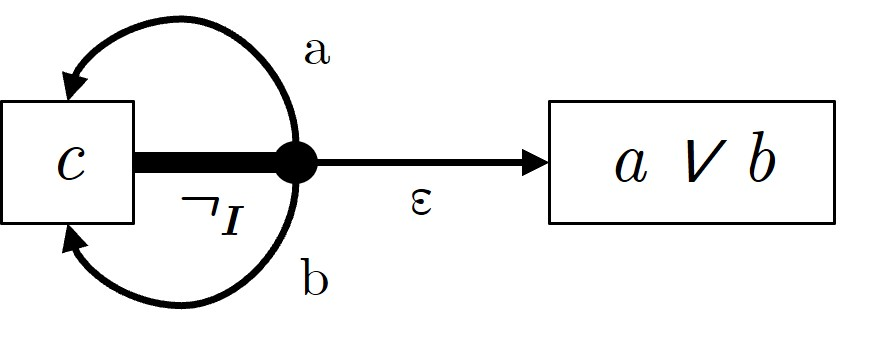
\includegraphics[width=\linewidth]{Chapters/Figures/te-pl-example.jpg}
\end{minipage}
 \caption{Example of a transition edge of \(\vee_E\) rule. Marks were ignored as irrelevant at this stage. The rule yields only two hypotheses, hence~$\varepsilon$ is needed.}
\label{fig:te-pl-ex}
\end{figure}

Formally, the above hyperedge is represented as $(c, \{(a \lor b, \varepsilon), (c, a), (c, b)\}, \vee_E)$. Edges go from the unique conclusion of the rule to its hypotheses. The labels of the heads of the hyperedge represent the possible additional hypothesis that can be used in that branch. In the above rule $\vee_E$, each side of the disjunction can be used as an additional hypothesis in the second and third branches of the rule, encoding the reasoning by cases, as explained in \autoref{rule:dis}.

The reason for using this type of graph is that it allows us to map rule applications directly into a data structure. Also, at this stage of the construction, there is no need to keep track of the marks. Later, we will show that these can be easily handled when extracting a solution from our algorithm.

To support \gls{FOL}, we must take into account more complex side conditions, such as those that depend on the open assumptions occurring in the rules \(\forall_I\) and \(\exists_E\) presented in \autoref{rule:uni} and \autoref{rule:exist}, respectively. It is necessary to keep track of the variables, since the system cannot guarantee that a rule application is correct at this stage of the algorithm, as the circumstances under which the rule was applied are not yet known. Unlike other side conditions, which can be directly verified when generating the edges, these variable-bounded conditions require explicit tracking. To represent these conditions, we defined a more complex head label, which, instead of containing only information about the generated hypothesis, also includes the variable that should not appear free in the rules \(\forall_I\) and \(\exists_E\). \autoref{fig:te-fol-ex} illustrates the formal construction of the \gls{TG} in \gls{FOL} by showing how the rule \(\exists_E\) can be represented as a hyperedge.

\begin{figure}[h!]
\centering
\begin{minipage}{0.45\textwidth}
    \centering
    \textbf{Rule application} \\[0.5em]
    \begin{prooftree}
      \AxiomC{$\overset{\displaystyle\mathcal{D}_1 \strut}{\exists x \; P(x)}$}
      \AxiomC{$\overset{\displaystyle\mathcal{D}_2 \strut}{\exists x \; Q(x)}$}
      \RightLabel{($\exists_E,\_$)}
      \BinaryInfC{$\forall x Q(x)$}
    \end{prooftree}
\end{minipage}
\hfill
\begin{minipage}{0.45\textwidth}
    \centering
    \textbf{Edge} \\[0.5em]
    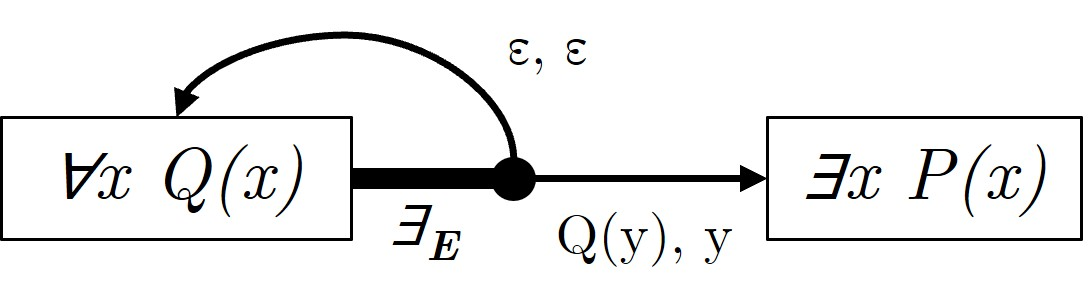
\includegraphics[width=\linewidth]{Chapters/Figures/te-fol-example.jpg}
\end{minipage}
        \caption{Example of a transition applied of \(\exists_E\) rule. Marks were ignored as irrelevant at this stage.}
\label{fig:te-fol-ex}
\end{figure}

In the rule $\exists_E$ above, we assume $Q(y)$ as a new hypothesis, obtained by substituting $x$ with $y$ in $Q(x)$. Following the side conditions, \(y\) cannot boccur free in any open assumptions of the derivation \(\mathcal{D}_2\). We encode the reasoning by cases by specifying which variable cannot appear free. Formally, the above hyperedge is represented as $(\forall x \, Q(x), \{(\exists x \, P(x), (Q(y), y)), (\forall x \, Q(x), (\varepsilon, \varepsilon))\}, \exists_E)$.

\subsubsection*{Procedure}
The first step in the construction of the \gls{TG}, called decomposition, is to compute its nodes. As recalled, the input consists of the main goal \(\Gamma \vdash \varphi\) and the target goal \(\Sigma \vdash \theta\), representing the problem and a partial proof provided by a user, respectively. The nodes are obtained by iterating through the formulas in the main and target goals. For each formula, we compute its set of sub-formulas and add them to the set of nodes. To handle more complex proofs that require reasoning by contradiction, we also include the negation of all these formulas. In this way, all formulas that can appear in a \gls{ND} proof of the problem are included as nodes in the \gls{TG}.

The decomposition step is crucial because it allows us to determine in advance which formulas will appear in the graph and to identify formulas that depend on this information. This is especially important for rules that can be applied to any formula, such as the \(\vee_E\) and \(\exists_E\) rules. The decomposition is performed by splitting each formula at its outermost logical operators, unless it is atomic. For example, the formula \(a \to \lnot b\) can be split into \(a\) and \(\lnot b\), whereas \(a\) cannot be decomposed since it is atomic. However, \(\lnot b\) can be further decomposed into \(b\). \autoref{alg:decomposition} shows the decomposition step where the nodes are computed.

\vspace{1em}
\begin{algorithm}[h]
\caption{Decomposition}
\label{alg:decomposition}
\KwIn{Main goal $\Gamma \vdash \varphi$, Target goal $\Sigma \vdash \theta$}
\KwOut{Set of formulas $F$}

$F \leftarrow \Gamma \cup \Sigma \cup \{\varphi, \theta\}$\tcp*[r]{Initialize formulas}

\ForEach{$f \in F$}{
  \If{$f$ was not already added as a negation}{
    $F \leftarrow F \cup \{\lnot f\}$\tcp*[r]{Add negation for indirect rules}
  }

  Decompose $f$ into parts $S$\tcp*[r]{The set of sub-formulae of $f$}
  $F \leftarrow F \cup S$\;
}

\end{algorithm}

The second and final step is to compute the hyperedges of the \gls{TG}. This is done by iterating over the set of formulas \(F\), and for each formula, assigning a set of rules based on the outermost logical symbol of the current formula. \autoref{alg:transitions} illustrates how each hyperedge is computed according to the corresponding rule. As previously mentioned, more complex rules, such as \(\vee_E\), require knowing in advance the list of formulas in order to create a hyperedge for each formula under consideration.

\begin{algorithm}[h]
\caption{Transitions}
\label{alg:transitions}
\KwIn{Set of formulas $F$}
\KwOut{Transition graph $T_G = (F, T_E)$}

$T_E \leftarrow \emptyset$\tcp*[r]{Initialize edges}

\ForEach{$f \in F$}{
    
    \If{$f$ was not added as a negation}{
        $T_E \leftarrow T_E \cup \{(f, \{(\bot, \lnot f)\}, \bot)\}$\;
    }

    \If{$f = \lnot \alpha$ for some $\alpha$}{
        $T_E \leftarrow T_E \cup \{(\lnot \alpha, \{(\bot, \alpha)\}, \lnot_I)\}$\;
        $T_E \leftarrow T_E \cup \{(\bot, \{(\alpha, \varepsilon), (\lnot \alpha,\varepsilon)\}, \lnot_E)\}$\;
    }

    \ElseIf{$f = \alpha \lor \beta$ for some $\alpha, \beta$}{
        $T_E \leftarrow T_E \cup \{(f, \{(\alpha, \varepsilon)\}, \vee_{I_R})\}$\;
        $T_E \leftarrow T_E \cup \{(f, \{(\beta, \varepsilon)\}, \vee_{I_L})\}$\;
        \ForEach{$f' \in F$}{
            $T_E \leftarrow T_E \cup \{(f', \{(f, \varepsilon), (f',\alpha), (f', \beta)\}), \vee_E\}$\;
        }
    }

    \ElseIf{$f = \alpha \land \beta$ for some $\alpha, \beta$}{
        $T_E \leftarrow T_E \cup \{(\alpha \land \beta, \{(\alpha, \varepsilon), (\beta,\varepsilon)\}, \land_{I})\}$\;
        $T_E \leftarrow T_E \cup \{(\alpha, \{(\alpha \land \beta, \varepsilon)\}, \land_{E_R})\}$\;
        $T_E \leftarrow T_E \cup \{(\beta, \{(\alpha \land \beta, \varepsilon)\}, \land_{E_L})\}$\;
    }

    \ElseIf{$f = \alpha \to \beta$ for some $\alpha, \beta$}{
        $T_E \leftarrow T_E \cup \{(\alpha \to \beta, \{(\beta, \alpha)\}, \to_{I})\}$\;
        $T_E \leftarrow T_E \cup \{(\beta, \{(\alpha, \varepsilon), (\alpha \to \beta, \varepsilon)\}, \to_{E})\}$\;
    }

}
\end{algorithm}

Although the first and second steps could be performed within a single loop, as it is possible to evaluate the outermost symbol of the current formula and assign the set of rules while extracting the subformulas, we have kept them separate for the sake of clarity and simplicity of presentation.

To support \gls{FOL} proofs, we must also account for the rules associated with quantifiers. To achieve this, we extend the decomposition step by tracking all terms \(T\) and variables \(V\) that can be extracted from the main and target goals. This tracking is essential because these terms and variables are used to generate new formulas through substitution, which in turn creates new nodes in the graph. 

By extending the rules in \autoref{alg:transitions} to include the quantifier rules, we can handle these additional symbols. For each rule, we consider substitutions using the previously computed terms \(T\) and variables \(V\), iterating through the respective sets and checking whether the resulting formula satisfies the required side conditions of the rule. This approach differs from the previous algorithm, where all nodes were computed during the decomposition step. Here, some nodes are generated dynamically along with the computation of the hyperedges. \autoref{alg:transitions-1} illustrates how the new hyperedges for \gls{FOL} rules are computed.

\begin{algorithm}
\caption{Transitions for FOL}
\label{alg:transitions-1}
\KwIn{Terms $T$, Variables $V$}

\If{$f = \forall \alpha\; \beta$ for some $\alpha \in V$ and $\beta$}{
    \ForEach{$t \in T$}{
        $f_m \gets Map(f, \alpha, t)$\tcp*[r]{Apply substitution of $\alpha$ by $t$ in $f$}
        \If{All side conditions of $\forall_E$ are satisfied}{
            $T_E \gets T_E \cup \{(f_m, \{(f, \varepsilon, \varepsilon)\}), \forall_E\}$\;
        }
    }
    \ForEach{$v \in V$}{
        $f_m \gets Map(f, \alpha, v)$\;
        \If{All side conditions of \(\forall_I\) that do not depend on the set of assumptions are satisfied}{
            $T_E \gets T_E \cup \{(f, \{(f_m, \varepsilon, v)\}), \forall_I\}$\;
        }
    }
}

\ElseIf{$f = \exists x\; \alpha$ for some $x \in V$ and $\alpha$}{
    \ForEach{$t \in T$}{
        $f_m \gets Map(f, \alpha, t)$\;
        \If{All side conditions of $\exists_I$ are satisfied}{
            $T_E \gets T_E \cup \{(f, \{(f_m, \varepsilon, \varepsilon)\}), \exists_I\}$\;
        }
    }
    \ForEach{$f' \in F$}{
        \ForEach{$v \in V$}{
            $f_m \gets Map(f, \alpha, v)$\;
            \If{All side conditions of $\exists_E$ that do not depend on the set of assumptions are satisfied}{
                $T_E \gets T_E \cup \{(f', \{(f, \varepsilon, \varepsilon), (f', f_m, v)\}), \exists_E\}$\;
            }
        }
    }
}
\end{algorithm}

\subsubsection*{Extending the \gls{TG} Construction Algorithm}
By keeping the \gls{TG} construction algorithm separate from the other steps, we can easily and conveniently manipulate the set of rules, allowing us to quickly add or modify rules without affecting other parts of the algorithm. As an example, if we want to add a new rule to the algorithm, such as the Transitivity of Implication rule (\(\to_\text{T}\)), the rule can be defined as follows:

\begin{minipage}{\linewidth}
\centering
\vspace{0.5cm}
\textbf{Elimination}
\begin{prooftree}
  \AxiomC{$\overset{\displaystyle\mathcal{D}_1 \strut} {\alpha \to \psi}$}
  \AxiomC{$\overset{\displaystyle\mathcal{D}_2 \strut} {\psi \to \beta}$}
  \RightLabel{$(\to_\text{T})$}
  \BinaryInfC{$\alpha \to \beta$}
\end{prooftree}
\end{minipage}
\vspace{0.2cm}

We only need to implement a new case to the implication branch of the algorithm with the instructions shown in \autoref{alg:tg-tu-rule}:

\begin{algorithm}[h]
\caption{Transitivity of Implication rule}
\label{alg:tg-tu-rule}

    \If{$f = \alpha \to \beta$ for some $\alpha, \beta$}{
        \ForEach{$f_l \in F$}{
            \If{$f_l = \alpha \to \psi$ for some $\psi$} {
                \ForEach{$f_r \in F$}{
                    \If{$f_r = \psi \to \beta$} {
                        $T_E = T_E \cup \{(\alpha \to \beta, \{(\alpha \to \psi, \varepsilon), (\psi \to \beta, \varepsilon)\}, \to_{T})\}$\;
                    }
                }
            }
        }
    }

\end{algorithm}

\subsubsection*{Examples}
We now present two examples, covering \gls{PL} and \gls{FOL}, illustrating how to construct the \gls{TG} step by step. To simplify the demonstrations, we do not consider proofs by contradiction, and thus we do not include the negation of each expression in the decomposition step.

\vspace{1em}
In the first example, we construct the \gls{TG} for the problem \(\{(p \to q) \to p\} \vdash q \to p\). Our main goal is to prove \(\{(p \to q) \to p\} \vdash q \to p\), and we assume that we aim to prove the full exercise, so the target goal is the same as the main goal. The first step is to compute the set \(F\) of formulas: by applying the decomposition, we obtain
\[
    F = \{(p \to q) \to p,\; p \to q,\; q \to p,\; p,\; q\}.
\]

Now, by iterating through all formulas in the set and matching them with the appropriate cases in order, we obtain the final \gls{TG} for the problem. 
\autoref{fig:tg-pl-ex-step-by-step} illustrates each step of the loop in the algorithm, following the order of the formulas in \(F\). 
In each step, the highlighted nodes correspond to the formulas currently being explored, and the highlighted edges represent the ones that were added. 
The last graph in the figure shows the complete \gls{TG} for the problem as constructed.

\begin{figure}[h]
    \centering
    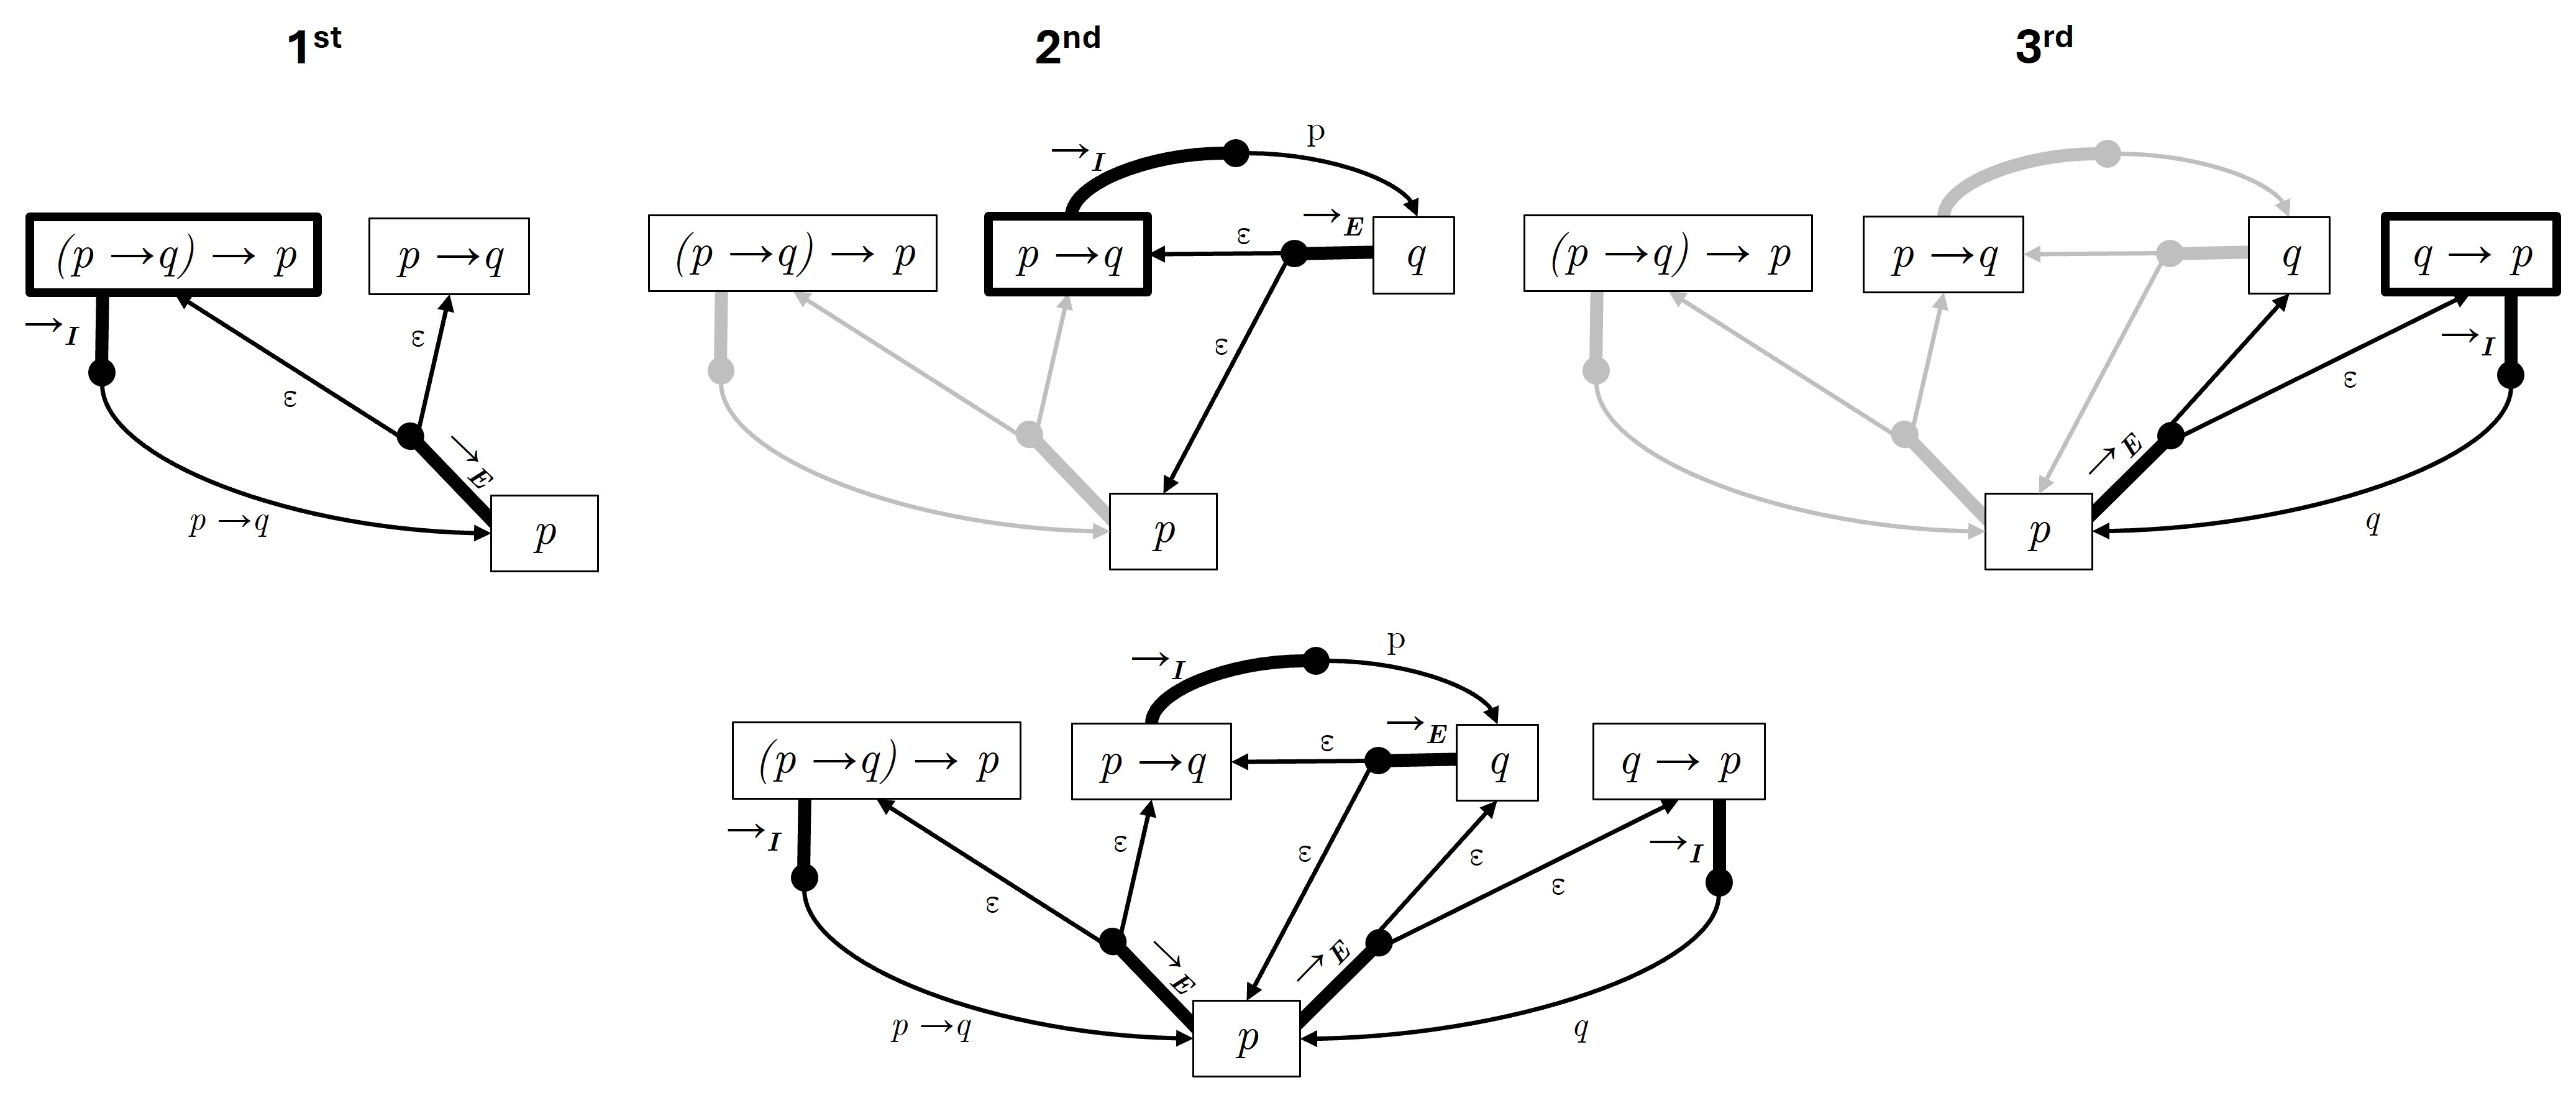
\includegraphics[width=1\linewidth]{Chapters/Figures/tg-pl-ex-step-by-step.jpg}
    \caption{Iteration of \autoref{alg:transitions} for the problem \(\{(p \to q) \to p\} \vdash q \to p\).}
    \label{fig:tg-pl-ex-step-by-step}
\end{figure}

\vspace{1em}
In the second example, our problem is \(\{\forall x\;(P(x) \land Q(x))\} \vdash \forall x\;P(x) \land \forall x\;Q(x)\), and we aim to prove \(\{\forall x\;(P(x) \land Q(x))\} \vdash \forall x\;Q(x)\). By computing the set of formulas \(F\) and keeping track of the terms \(T\) and variables \(V\), we obtain:
\[
\begin{aligned}
F &= \bigl\{ \forall x\,P(x) \land \forall x\,Q(x),\;\; \forall x\,P(x),\;\; \forall x\,Q(x),\;\; \forall x\,(P(x) \land Q(x)),\\
&\quad P(x) \land Q(x),\;\; P(x),\;\; Q(x) \bigr\},\\[2mm]
T &= \{x\}, \qquad V = \{x\}.
\end{aligned}
\]

Finally, iterating over the set of formulas we construct the \gls{TG}. \autoref{fig:tg-fol-ex-step-by-step} shows step by step how the different hyperedges were added.

\begin{figure}[h]
    \centering
    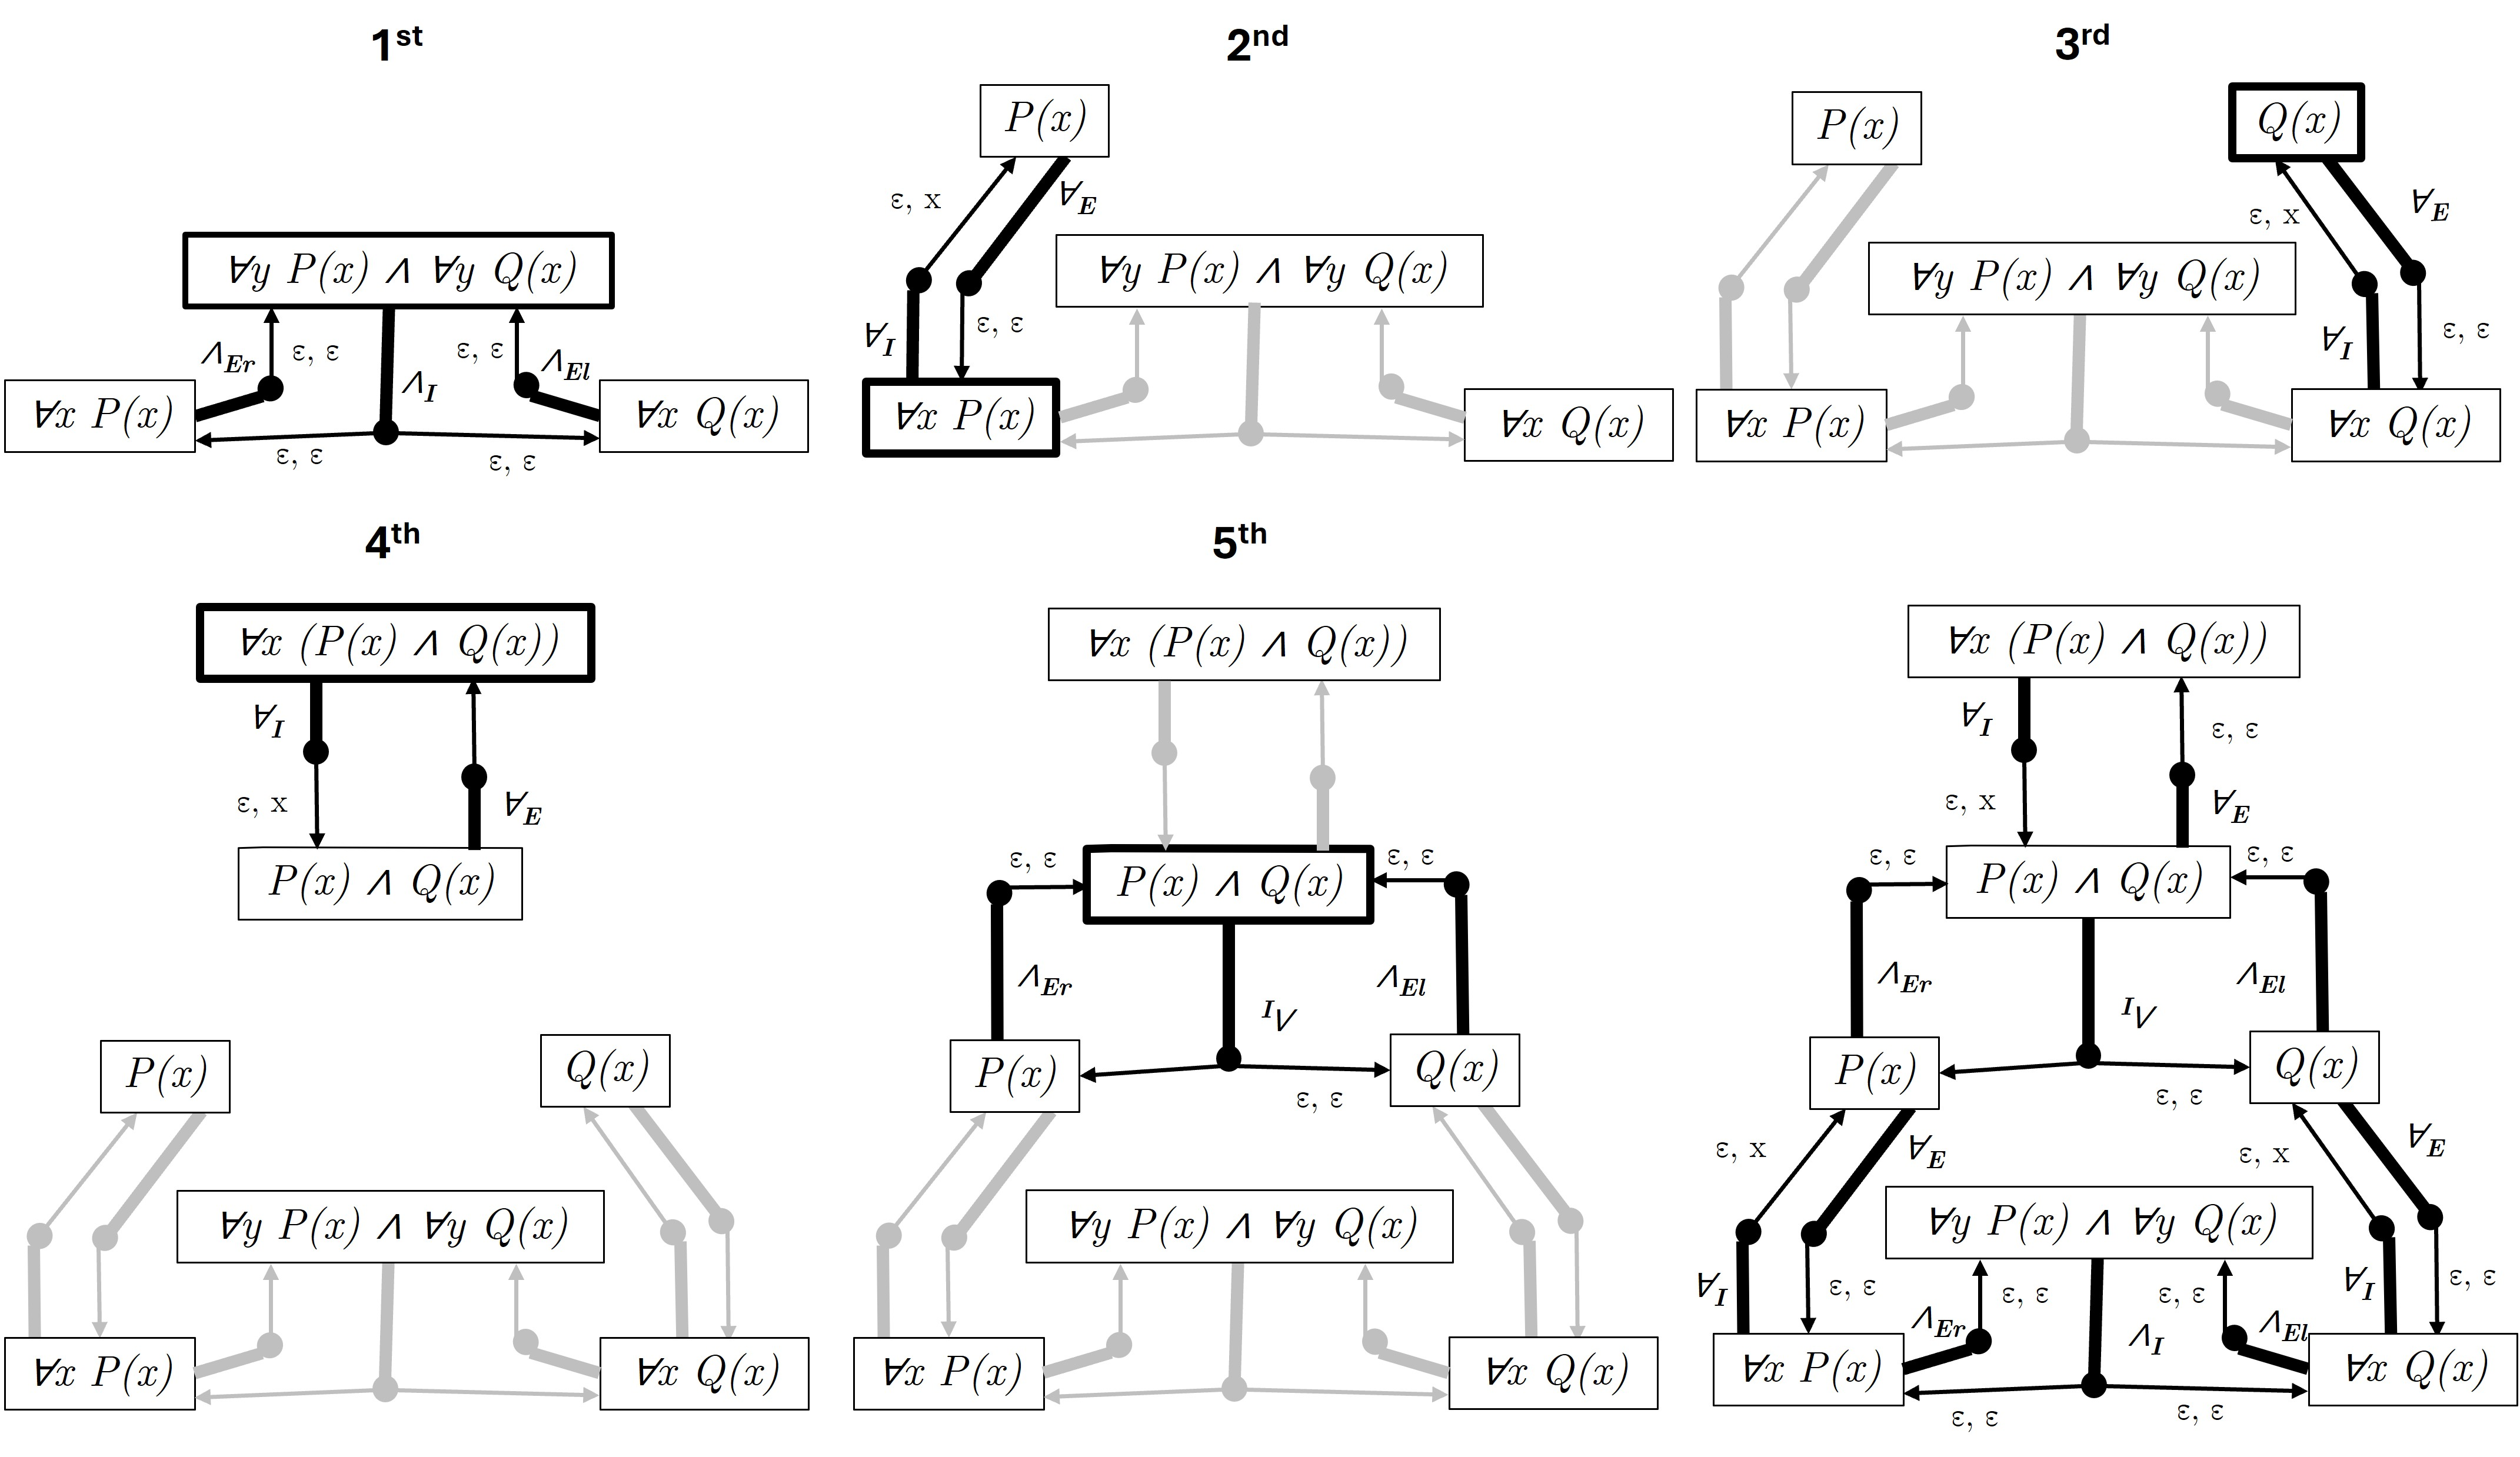
\includegraphics[width=1\linewidth]{Chapters/Figures/tg-fol-ex-step-by-step.jpg}
    \caption{Iteration of \autoref{alg:transitions} together with \autoref{alg:transitions-1} for the main goal \(\{\forall x\;(P(x) \land Q(x))\} \vdash \forall x\;P(x) \land \forall x\;Q(x)\) and the target goal \(\{\forall x\;(P(x) \land Q(x))\} \vdash \forall x\;Q(x)\).}
    \label{fig:tg-fol-ex-step-by-step}
\end{figure}

\subsection{Proof Graph}
The second step is to build the \gls{PG}. The construction of a \gls{PG} follows a similar reasoning to the \gls{TG}, but it is defined on goals. It contains all possible sub-goals derived from the target goal. In this graph, nodes are goals, and edges are adaptations of \gls{TE} that now refer to goals. 

The purpose of this graph is to decompose the target goal into smaller goals that are easier to prove, until we reach goals that can be directly proved. In the end, after generating all sub-goals, the graph may contain multiple proof paths. 

Some of these paths may not lead to a solution, while others may succeed in proving the target goal. In short, the \gls{PG} aims to find the maximum number of different ``game'' combinations using the "moves" generated in the \gls{TG}. To generate the \gls{PG}, we use the \gls{TG}, previously generated, and the target goal. Before we describe the procedure, we define some key terms:

\begin{definition}[Proof Graph]
\label{def:pg}
A \emph{Proof Graph} is a pair $P_G = (G, P_E)$:
\begin{itemize}[noitemsep]
  \item \( G \) is a finite set of \emph{goals}, and
  \item \( P_E \subseteq G \times \mathcal{P}(G) \times R \) is a finite set of \emph{labeled hyperedges} called \emph{\gls{PE}}, where each edge consists of:
  \begin{itemize}[noitemsep]
    \item a tail goal \( g \in G \),
    \item a set of goals, and
    \item a rule \( r \in R \).
  \end{itemize}
\end{itemize}
\end{definition}

\begin{definition}[Proved Goal]
A goal \( \Delta \vdash \delta \) is \emph{proved} if either:
\begin{itemize}[noitemsep]
  \item \( \delta \in \Delta \), or
  \item there exists a Proof Edge \( (g, T, r) \in P_E \) in the Proof Graph \( P_G = (G, P_E) \), such that \( g = \Delta \vdash \delta \), and for every goal in \(T\), the goal is proved.
\end{itemize}
\end{definition}

The definition of proved goal is extremely important because it is used as a stopping condition to avoid the algorithm looping through unnecessary goals and to guarantee that the proof is valid. This is only possible due to the type of graph chosen, as it allows us to capture the relation between the hypotheses and the conclusion of each rule application. \autoref{fig:pe-ex} shows an example of a \gls{PE} and how these relations can be captured. 
\begin{figure}[h!]
\centering
\begin{minipage}{0.45\textwidth}
    \centering
    \textbf{Rule application}\\
    {\fontsize{10pt}{10pt}\selectfont \textbf{Goal:} \(\{a \vee b\} \vdash a\)}
    \begin{prooftree}
      \AxiomC{$a \vee b$}
      \AxiomC{${a}^2$}
      \AxiomC{$a$}
      \RightLabel{($\vee_E, 2, \_$)}
      \TrinaryInfC{$a$}
    \end{prooftree}
\end{minipage}
\hfill
\begin{minipage}{0.45\textwidth}
    \centering
    \textbf{Edge} \\[0.5em]
    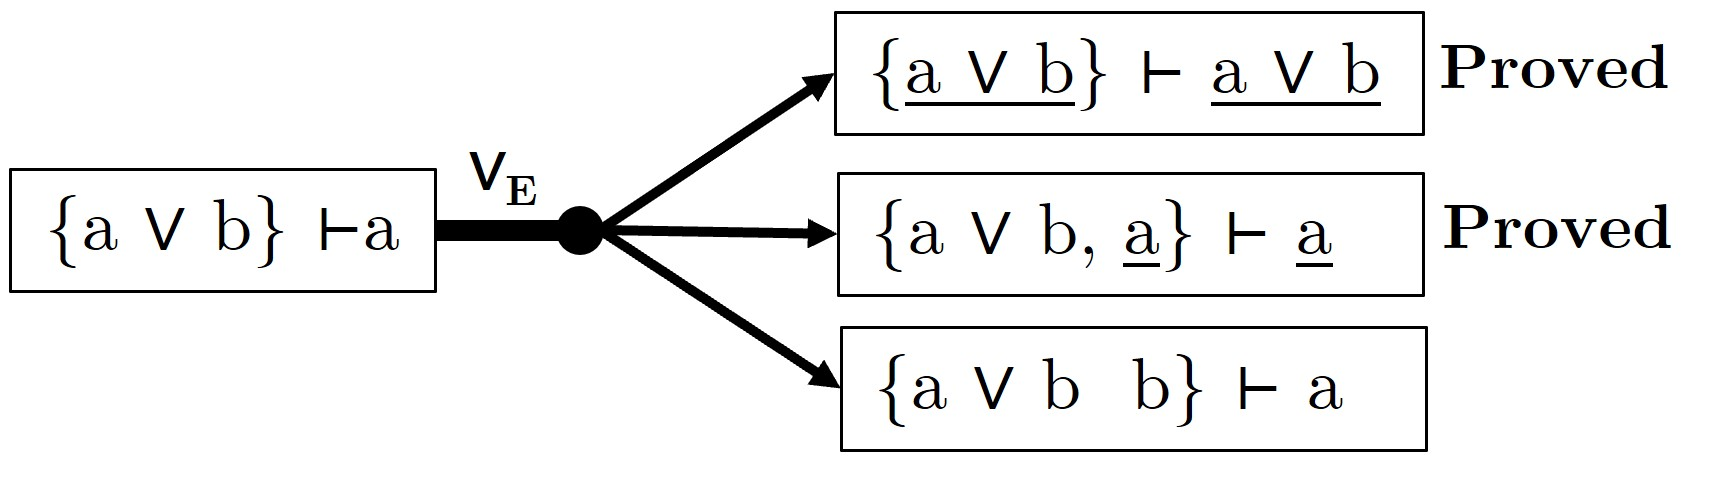
\includegraphics[width=1\linewidth]{Chapters/Figures/pe-example.jpg}
\end{minipage}
        \caption{Proof attempt of $\{a \lor b\} \vdash a$, no valid proof found.}
\label{fig:pe-ex}
\end{figure}

%For \gls{FOL} problems, the overall logic remains the same, however, it is necessary to introduce a small modification to the goal object by including a list of variables that cannot appear free in the open hypotheses, thereby ensuring that only valid solutions are captured. \autoref{fig:pe-ex-fol} presents an example of a proof attempt in \gls{FOL}.

In the figure, we want to prove \(\{a \vee b\} \vdash a\). By applying the Elimination of Disjunction rule (\(\exists_E\)), we notice that one of the hypotheses cannot be closed using only this rule, even if the other two hypotheses are closed. So, what we actually prove with this rule is \(\{a \vee b, a\} \vdash a\), which is different from our goal. To accurately track proved goals and only valid proved goals, we must organize goals in a hypergraph structure.
%Another example, this time in \gls{FOL}, is shown in \autoref{fig:pe-ex-fol}, where \(Q(y)\) was taken as an assumption.

%\begin{figure}[h!]
%\centering
%\begin{minipage}{0.35\textwidth}
%    \centering
%    \textbf{Rule application}\\
%    {\fontsize{10pt}{10pt}\selectfont \textbf{Goal:} \(\{\exists x \;P(x)\} \vdash \forall x \; Q(x)\)}
%    \begin{prooftree}
%      \AxiomC{$\exists x \; P(x)$}
%      \AxiomC{$\forall x \; Q(x)$}
%      \RightLabel{($\exists_E,\_$)}
%      \BinaryInfC{$\forall x Q(x)$}
%    \end{prooftree}
%\end{minipage}
%\hfill
%\begin{minipage}{0.55\textwidth}
%    \centering
%    \textbf{Edge} \\[0.5em]
%    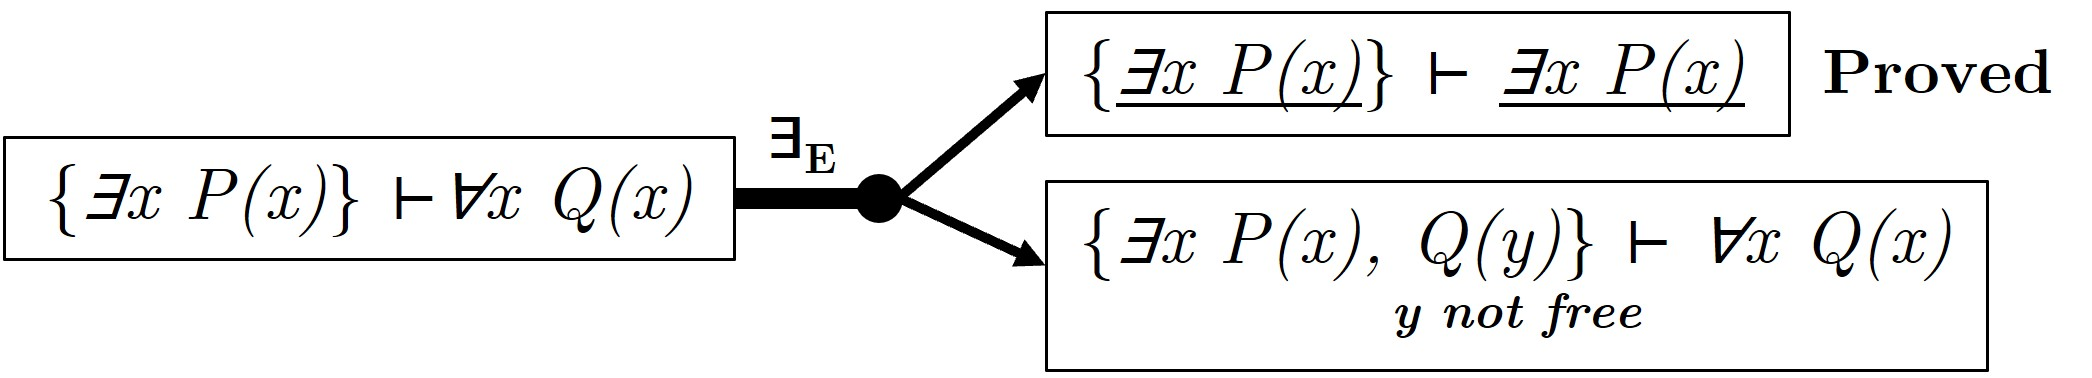
\includegraphics[width=1\linewidth]{Chapters/Figures/pe-example-fol.jpg}
%\end{minipage}
%        \caption{Proof attempt of $\{\exists x \;P(x)\} \vdash \forall x \; Q(x)$, no valid proof found. Assuming assumption \(Q(y).\)}
%\label{fig:pe-ex-fol}
%\end{figure}

\subsubsection*{Procedure}
With all the necessary definitions in place, we now present the procedure to generate the \gls{PG}, as shown in \autoref{alg:pg-construction}.

\begin{algorithm}
\caption{Proof Graph}
\label{alg:pg-construction}
\KwIn{Transition Graph $T_G = (F, T_E)$, Target goal $t_\text{goal}$}
\KwOut{Proof Graph $P_G = (G, P_E)$}

$G \leftarrow \{t_\text{goal}\}$\tcp*[r]{Initialize set of goals}
$P_E \leftarrow \emptyset$\tcp*[r]{Initialize set of proof edges}

\tcp{Compute sub-goals}
\ForEach{$g = \Sigma \vdash \theta \in G$}{

    \If{$g$ is proved}{
        \textbf{continue}\tcp*[r]{Skip proved goal}
    }

    \If{stopping condition is reached}{
        \textbf{break}\tcp*[r]{Avoid excessive expansion}
    }

    \tcp{Get transition edges for formula $\theta$}
    $TE_\theta \leftarrow \{ (f, H, r) \in T_E \mid f = \theta \}$\;

    \ForEach{$(f, H, r) \in TE_\theta$}{
        $T \leftarrow \emptyset$\tcp*[r]{Store transitions to each hypothesis}
        
        \ForEach{$(f_1, f_2) \in H$}{
            \tcp{Create sub-goal by extending the current premises with the closed hypothesis}
            $g_\text{new} \leftarrow (\Sigma \cup \{f_2\}) \vdash f_1$\;

            $T \leftarrow T \cup \{g_\text{new}\}$\;
            $G \leftarrow G \cup \{g_\text{new}\}$\tcp*[r]{Add sub-goal to the loop}
        }

        $P_E \leftarrow P_E \cup \{(g, T, r)\}$\tcp*[r]{Add proof edge}
    }
}
\end{algorithm}

This algorithm generates very large graphs, with numerous distinct goals depending on the complexity of the problem, especially when dealing with \gls{FOL}, as it is undecidable. In a pedagogical context, since the size of the proofs we are considering is small, it is not necessary to explore the entire goal space, as many goals are extremely complex and do not provide useful feedback. Therefore, stopping conditions are required, and these depend on the complexity of the specific exercise. These may include limiting the total number of goals explored, setting a maximum number of hypotheses allowed per goal, or enforcing a timeout. The algorithm will always find a solution if the problem is solvable and no limits are set, but it might take a lot of time and memory.

To handle \gls{FOL} problems, we must check whether the goals we are transitioning to are valid before adding them to the list of goals to be explored. By \emph{valid}, we mean goals that satisfy the side condition of having no open assumptions in the derivation. 
At this stage of the algorithm, we have access to the list of assumptions made at a given point in the proof (stored in the goals), so we can verify whether the side condition is satisfied. When a rule that introduces such a restriction is applied in the \gls{PG}, we can check whether the bounded variable present in the target expression of that rule is free in the premises of our current goal. 
In other words, let us assume that our current goal, the one currently being explored by the algorithm, is \(\Sigma \vdash \theta\), and suppose that there is a \gls{TE} with a rule that has a bound variable \(y\). If, for all assumptions in \(\Sigma\), the variable \(y\) is not free, then we can conclude that the goal is valid. This holds because the environment of assumptions to be considered is the one that existed prior to the application of the rule.

\vspace{-0.5cm}

\subsubsection*{Examples}
Following the same two examples presented during the \gls{TG} construction, we now present the construction of the corresponding \gls{PG}.

\vspace{1em}
In the first example, by applying the procedure illustrated in \autoref{fig:tg-pl-ex-step-by-step} to our target goal, we obtain the \gls{PG}. \autoref{fig:st-ex} shows the step-by-step construction of the graph. In this example, the entire space of goals is explored. However, when considering more complex problems, especially when including the negation of formulas, the \gls{PG} can become extremely large if appropriate stopping conditions are not defined. 
Although it may seem unusual to keep multiple solutions for the same problem in a single graph, this is a deliberate design choice in our algorithm. By sacrificing memory usage, we can provide faster feedback, resulting in a more responsive system. Later in this chapter, this trade-off will be discussed in greater detail. The final result for this example is shown in \autoref{fig:st-ex-final}.

\begin{figure}[h]
    \centering
    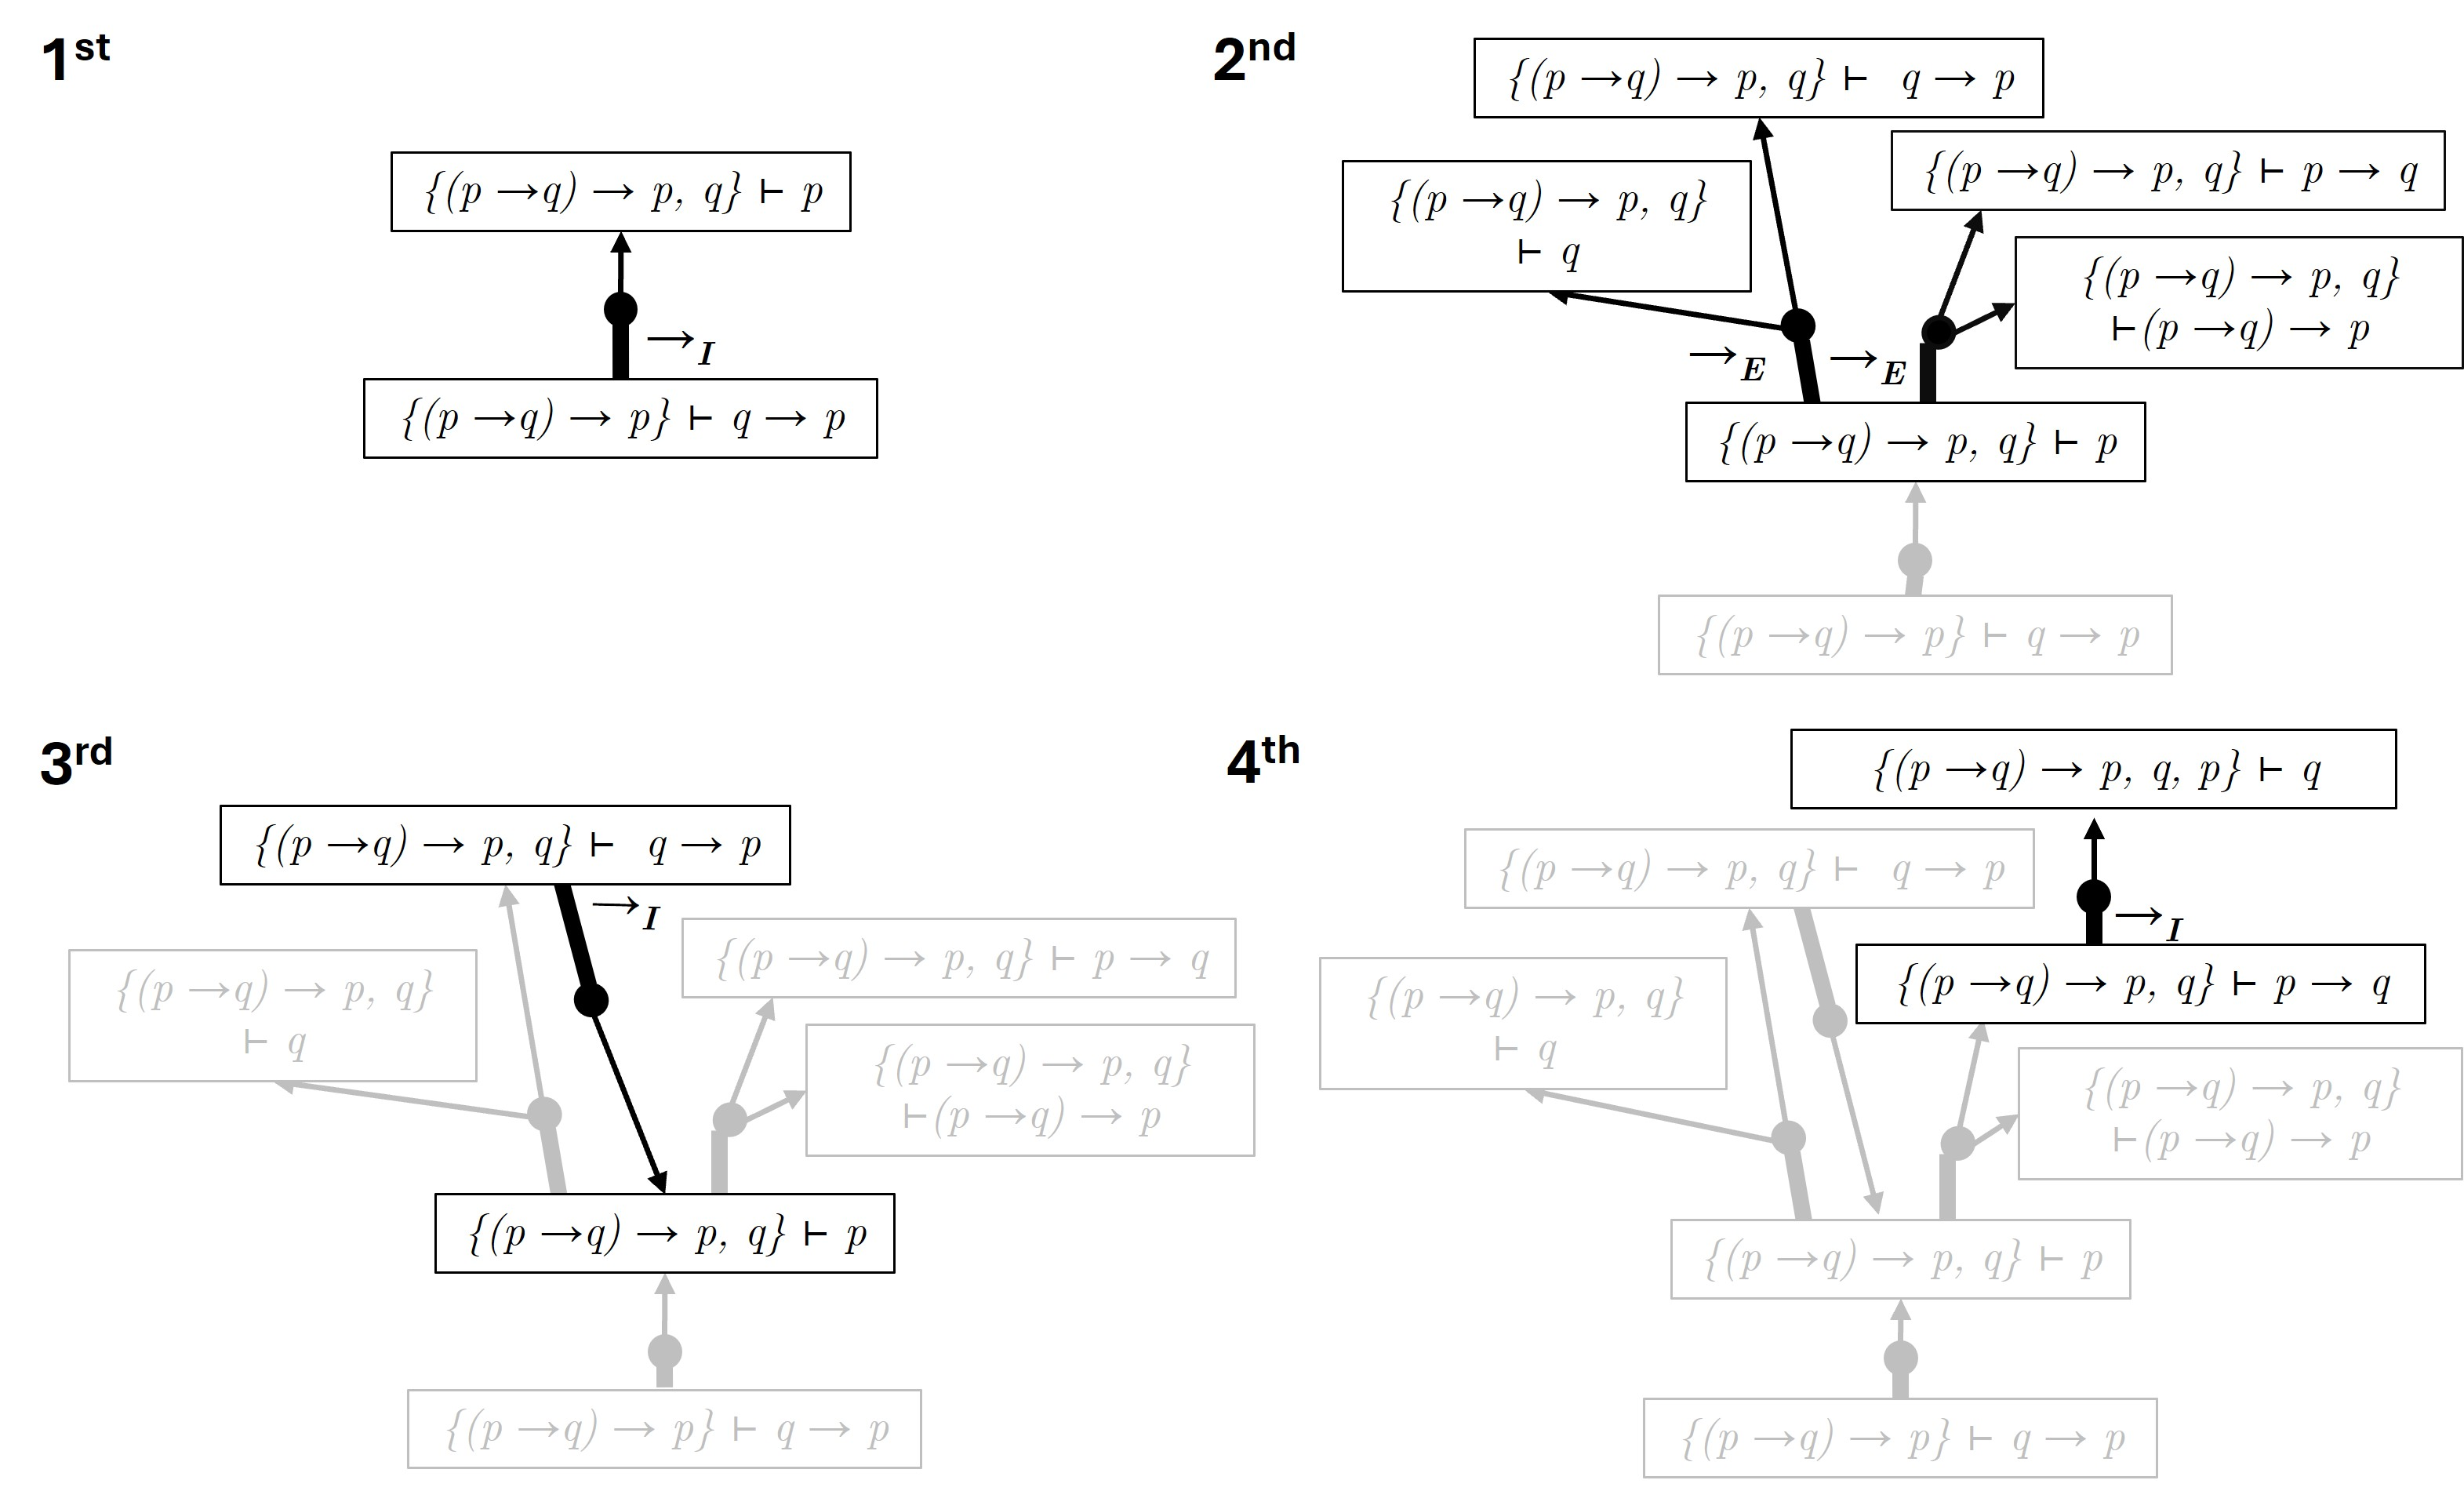
\includegraphics[width=1\linewidth]{Chapters/Figures/sg-gen.jpg}
    \caption{Step-by-step construction of a PG using the \autoref{alg:pg-construction} and the TG from \autoref{fig:tg-pl-ex-step-by-step}. }
    \label{fig:st-ex}
\end{figure}
\vspace{1em}
\begin{figure}[h]
    \centering
    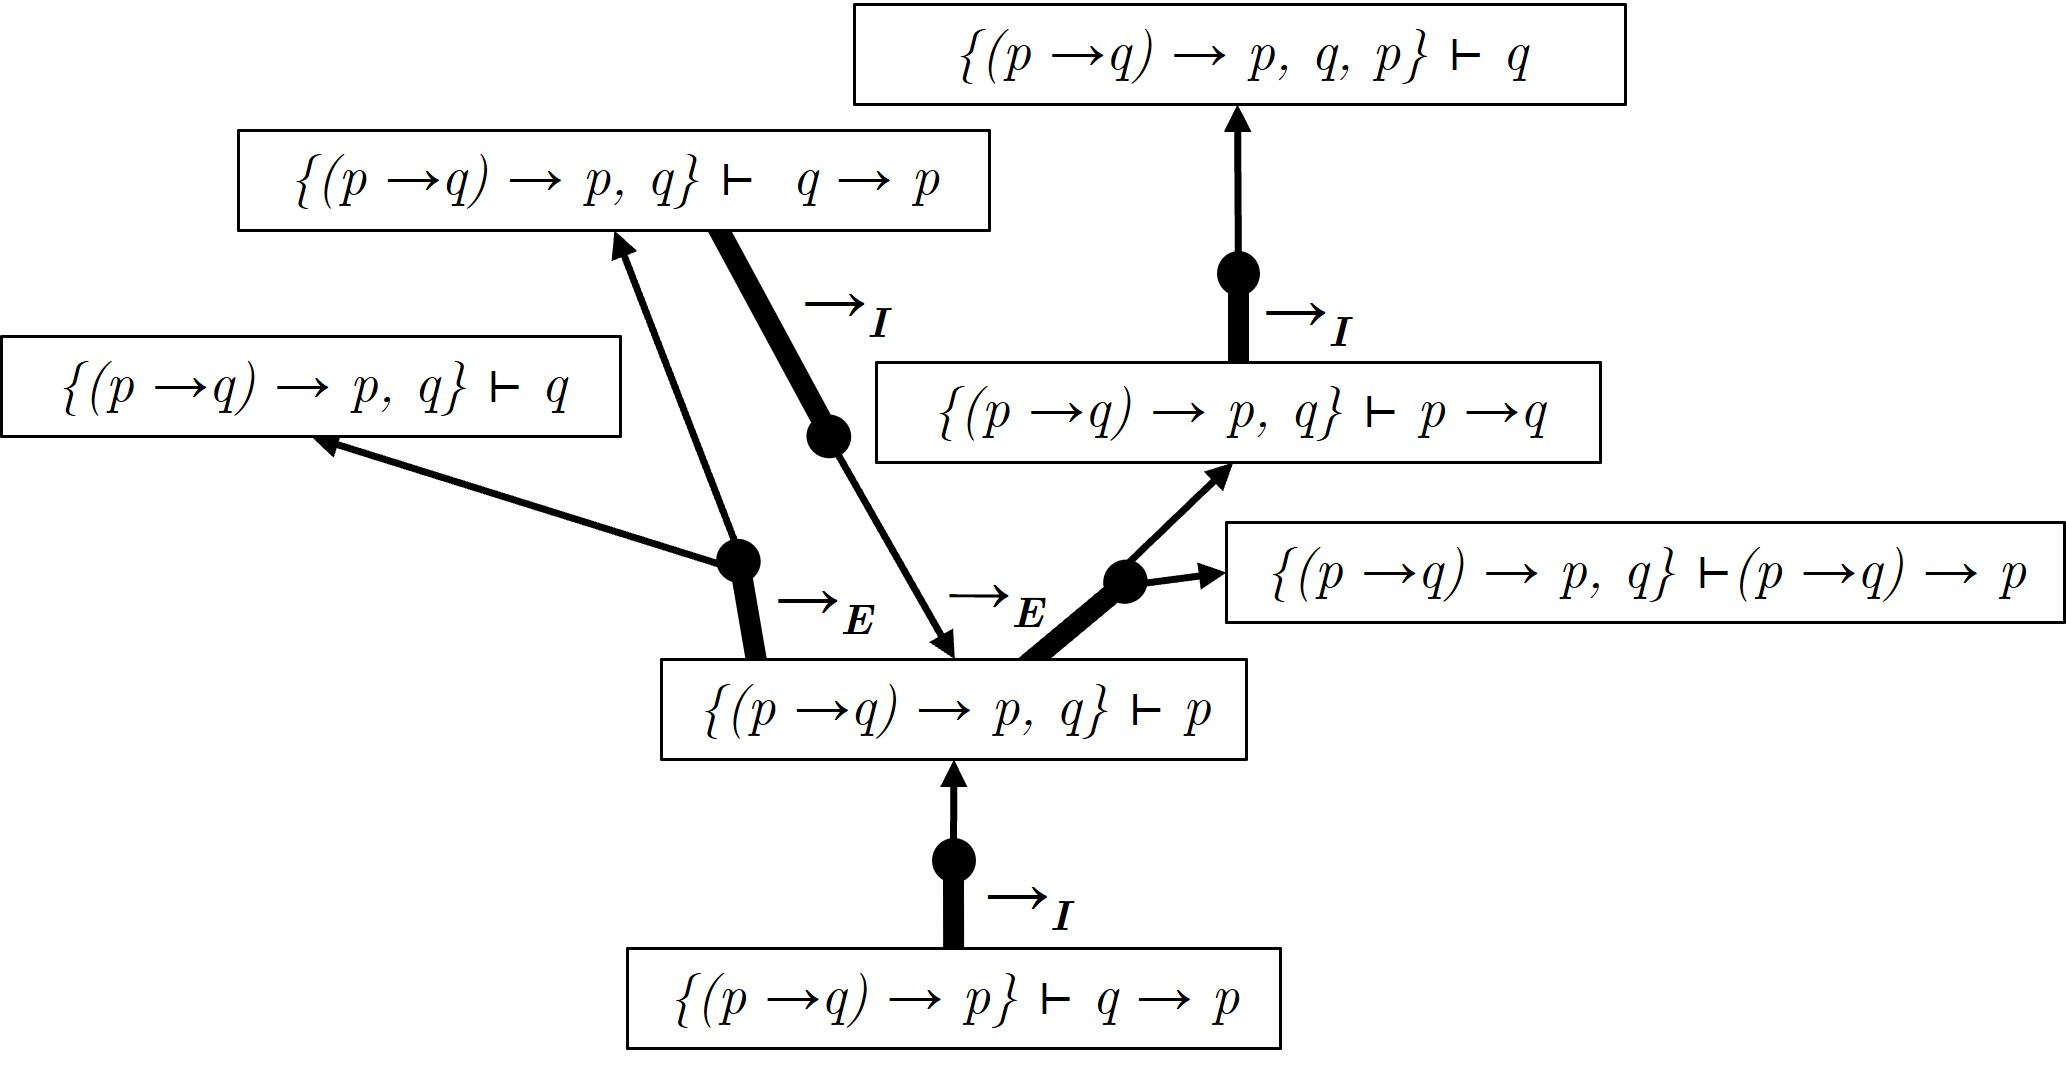
\includegraphics[width=0.8\linewidth]{Chapters/Figures/sg-ex-final.jpg}
    \caption{Final PG obtained from the TG shown in \autoref{fig:tg-pl-ex-step-by-step}}
    \label{fig:st-ex-final}
\end{figure}

For the second example, the step-by-step construction is not shown. However, by applying the same algorithm and taking into account the \emph{validity} of the explored goals, we can obtain the final \gls{PG} presented in \autoref{fig:st-ex-fol-final}.

\begin{figure}[h]
    \centering
    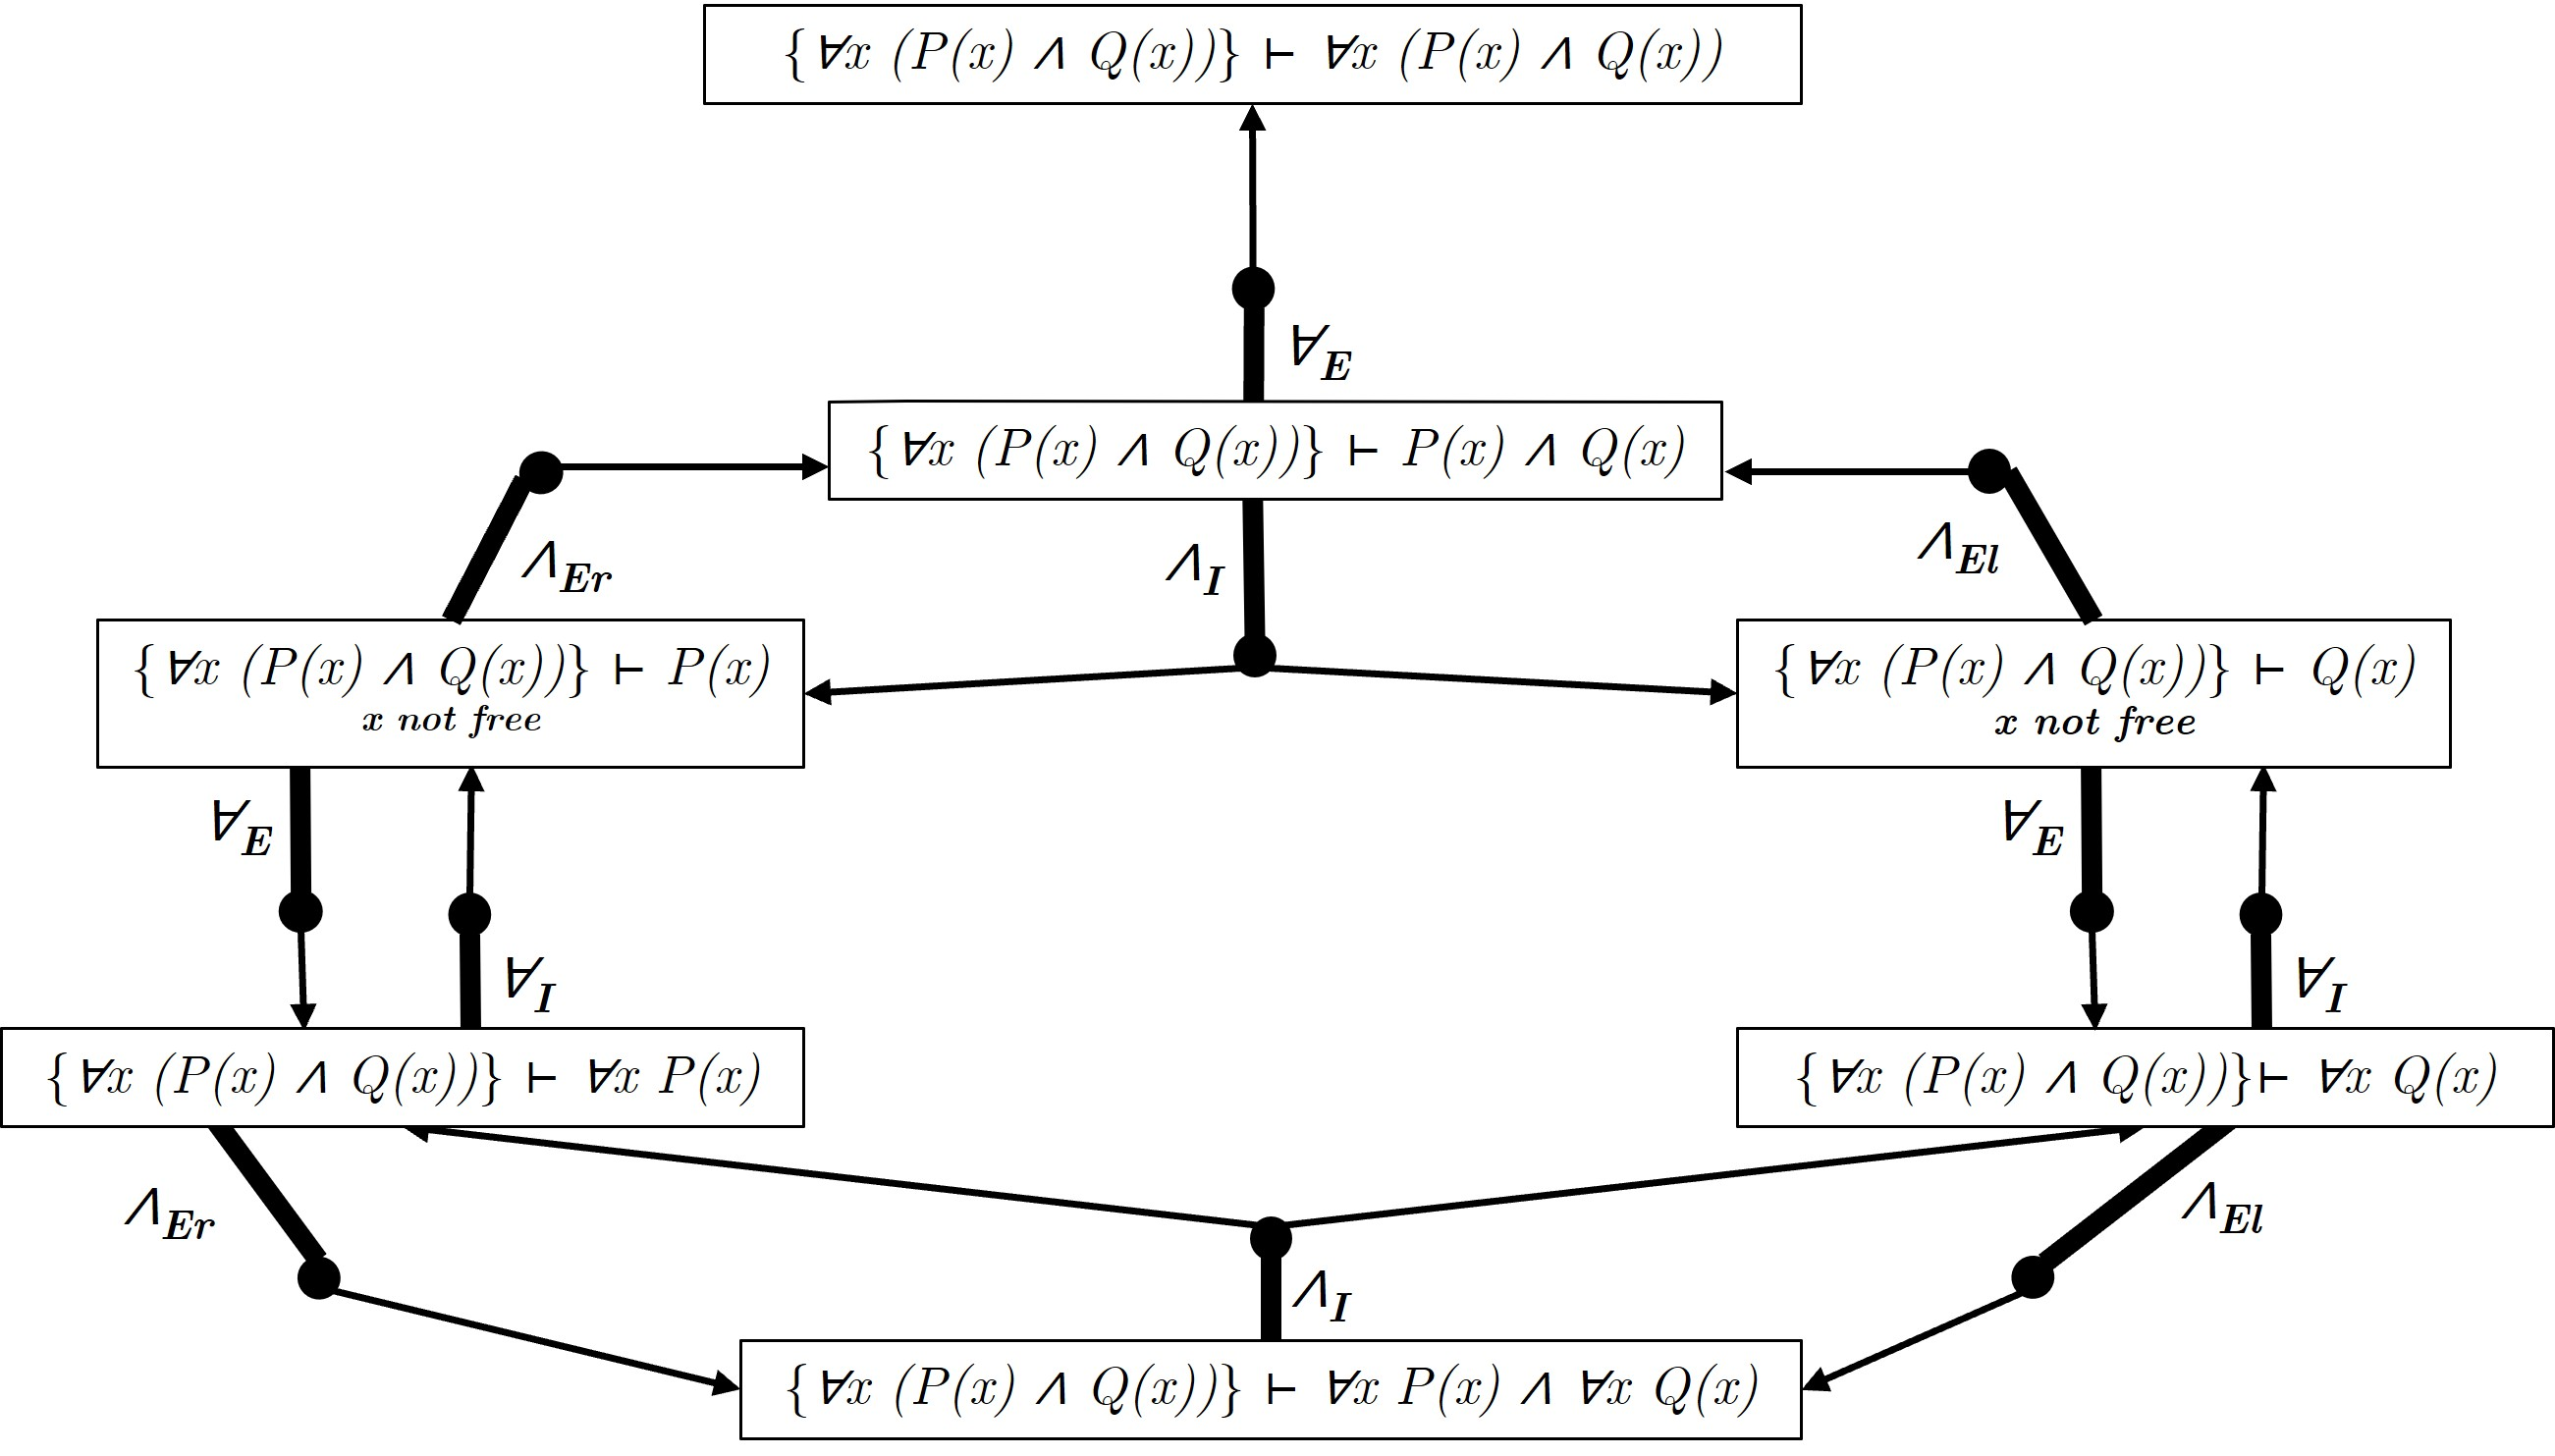
\includegraphics[width=0.8\linewidth]{Chapters/Figures/sg-ex-fol-final.jpg}
    \caption{Final PG obtained from the TG shown in \autoref{fig:tg-fol-ex-step-by-step}.}
    \label{fig:st-ex-fol-final}
\end{figure}

In the \gls{PG}s presented above, all states are \emph{proved}, meaning that there is no path to a solution that ends in a dead end (does not solve the target goal). Such dead ends may occur in more complex problems, where the graph becomes larger, or when the algorithm terminates prematurely due to the stopping conditions.

\subsection{Trimmed Proof Graph}
The final stage of our algorithm consists of trimming the \gls{PG} to keep only the solutions of the problem creating the \gls{TPG}. In our analogy this corresponds to the step where we choose the best set of ``moves'' that lead to a win. Let us first analyze the two \gls{PG}s previously computed. From those graphs we can extract numerous solutions, in fact there are infinitely many of them. If we take a closer look we can notice that in both graphs there are loops, which means that we can repeat those rules infinitely to generate new and different proofs. \autoref{fig:sol-pg-pl} and \autoref{fig:sol-pg-fol} present some examples of proofs that can be extracted from the \gls{PG}s. For simplicity, marks were omitted.

\begin{figure}[ht]
\centering
\small
\begin{minipage}{0.44\linewidth}
\centering
\begin{prooftree}
  \AxiomC{$q$}
  \RightLabel{$(\to_I)$}
  \UnaryInfC{$p \to q$}
  
  \AxiomC{$(p \to q) \to p$}
  
  \RightLabel{$(\to_E)$}
  \BinaryInfC{$p$}
  \RightLabel{$(\to_I)$}
  \UnaryInfC{$q \to p$}
\end{prooftree}
\end{minipage}%
\hfill
\begin{minipage}{0.01\linewidth}
\centering
\rule{0.4pt}{2.5cm} % vertical line: width x height
\end{minipage}%
\hfill
\begin{minipage}{0.52\linewidth}
\centering
\begin{prooftree}
  \AxiomC{$q$}
  
  \AxiomC{$q$}
  \RightLabel{$(\to_I)$}
  \UnaryInfC{$p \to q$}
  
  \AxiomC{$(p \to q) \to p$}
  
  \RightLabel{$(\to_E)$}
  \BinaryInfC{$p$}
  \RightLabel{$(\to_I)$}
  \UnaryInfC{$q \to p$}
  
  \RightLabel{$(\to_E)$}
  \BinaryInfC{$p$}
  \RightLabel{$(\to_I)$}
  \UnaryInfC{$q \to p$}
\end{prooftree}
\end{minipage}
\caption{Some examples of proofs extracted from \autoref{fig:st-ex-final} }
\label{fig:sol-pg-pl}
\end{figure}

\begin{figure}[ht]
\centering
\small

\begin{prooftree}

\AxiomC{$\forall x \,(P(x) \land Q(x))$}
\RightLabel{$(\forall_E$}
\UnaryInfC{$P(x) \land Q(x)$}
\RightLabel{$(\land_{E_r})$}
    \UnaryInfC{$P(x)$}
    \RightLabel{$(\forall_I)$}
  \UnaryInfC{$\forall x \, P(x)$}

  \AxiomC{$\forall x \,(P(x) \land Q(x))$}
\RightLabel{$(\forall_E$}
\UnaryInfC{$P(x) \land Q(x)$}
\RightLabel{$(\land_{E_l})$}
    \UnaryInfC{$Q(x)$}
    \RightLabel{$(\forall_I)$}
  \UnaryInfC{$\forall x \, Q(x)$}
  
  \RightLabel{$(\land_I)$}
  \BinaryInfC{$\forall x \, P(x) \land \forall x \, Q(x)$}
\end{prooftree}
\caption{Example of a proof extracted from \autoref{fig:st-ex-fol-final} }
\label{fig:sol-pg-fol}
\end{figure}

To obtain a solution from the \gls{PG} we start from the target node, the one used to begin the generation of solutions, and from there we select a path until a leaf is reached. However, reaching a leaf does not guarantee a valid solution. Let us suppose that the number of nodes explored during the generation of the \gls{PG} was limited. In this case, some of the leaf nodes are considered \emph{proved}, while others are not because the algorithm stopped prematurely. The goal of this step is therefore to remove the nodes that are not \emph{proved} and, at the same time, to keep only the edges that lead to the shortest proofs. In other words, the final graph will contain only \emph{proved} goals, and each goal will have at most one outgoing edge that leads to the shortest solution found.
The definition of shortest proofs can be interpreted in two different ways: one based on height (Height Trim Strategy), and the other based on the number of formulas involved (Size Trim Strategy). Our algorithm supports both strategies, which rely on a standard graph traversal technique, namely \emph{breadth-first search} and \emph{uniform cost search}, to determine which nodes and edges should be preserved.

\subsubsection*{Height Trim Strategy} 
The \gls{HTS} algorithm traverses the \gls{PG} in reverse order: it starts from the leaves and visits nodes using \emph{breadth-first search} algorithm. Since this traversal guarantees that each node is first reached through the shortest possible path in terms of height, the algorithm retains only the first \gls{PE} that reaches each goal. All other incoming edges to the same goal are discarded, even if alternative solutions with the same height exist. \autoref{fig:sg-trim-height} illustrates step by step how the \gls{HTS} is applied to the \gls{PG} presented in \autoref{fig:st-ex-final}. Red edges indicate those that were removed, and the highlighted portion of the graph in each step represents the part of the \gls{PG} that has already been trimmed.

\vspace{0.5em}
\textbf{Steps:}

\begin{enumerate}
    \item[\textbf{\ordinalnum{1}}] The algorithm attempts to explore the incoming edges of the goal \(\{(p \to q) \to p, q\} \vdash q\). Since the only incoming edge has multiple heads and one of the heads has not yet been explored, namely \(\{(p \to q) \to p, q\} \vdash q \to p\), the algorithm skips to the next goal. 
    
    \item[\textbf{\ordinalnum{2}}] The goal \(\{(p \to q) \to p, q, p\} \vdash q\) is explored. Its only incoming edge has itself as a head, which was already explored. Therefore, the algorithm adds the tail goal of that edge, \(\{(p \to q) \to p, q\} \vdash p \to q\), to the set of goals to be explored. 
    
    \item[\textbf{\ordinalnum{3}}] The algorithm explores the goal \(\{(p \to q) \to p, q\} \vdash (p \to q) \to p\), but encounters the same case as in step~\ordinalnum{1}. It then proceeds to the goal \(\{(p \to q) \to p, q\} \vdash p \to p\). This time all heads of the incoming edge have already been explored, so the tail goal \(\{(p \to q) \to p, q\} \vdash p\) is added to the set of goals to be explored, and the other edges originating from it are removed from the graph. 
    
    \item[\textbf{\ordinalnum{4}}] In the final step the goal \(\{(p \to q) \to p, q\} \vdash p\) is explored. All incoming edges have explored heads. Since the tail goals of these edges have no incoming edges, they can be marked automatically as explored. As there are no more goals left to explore, the algorithm terminates.
\end{enumerate}

\begin{figure}[h]
    \centering
    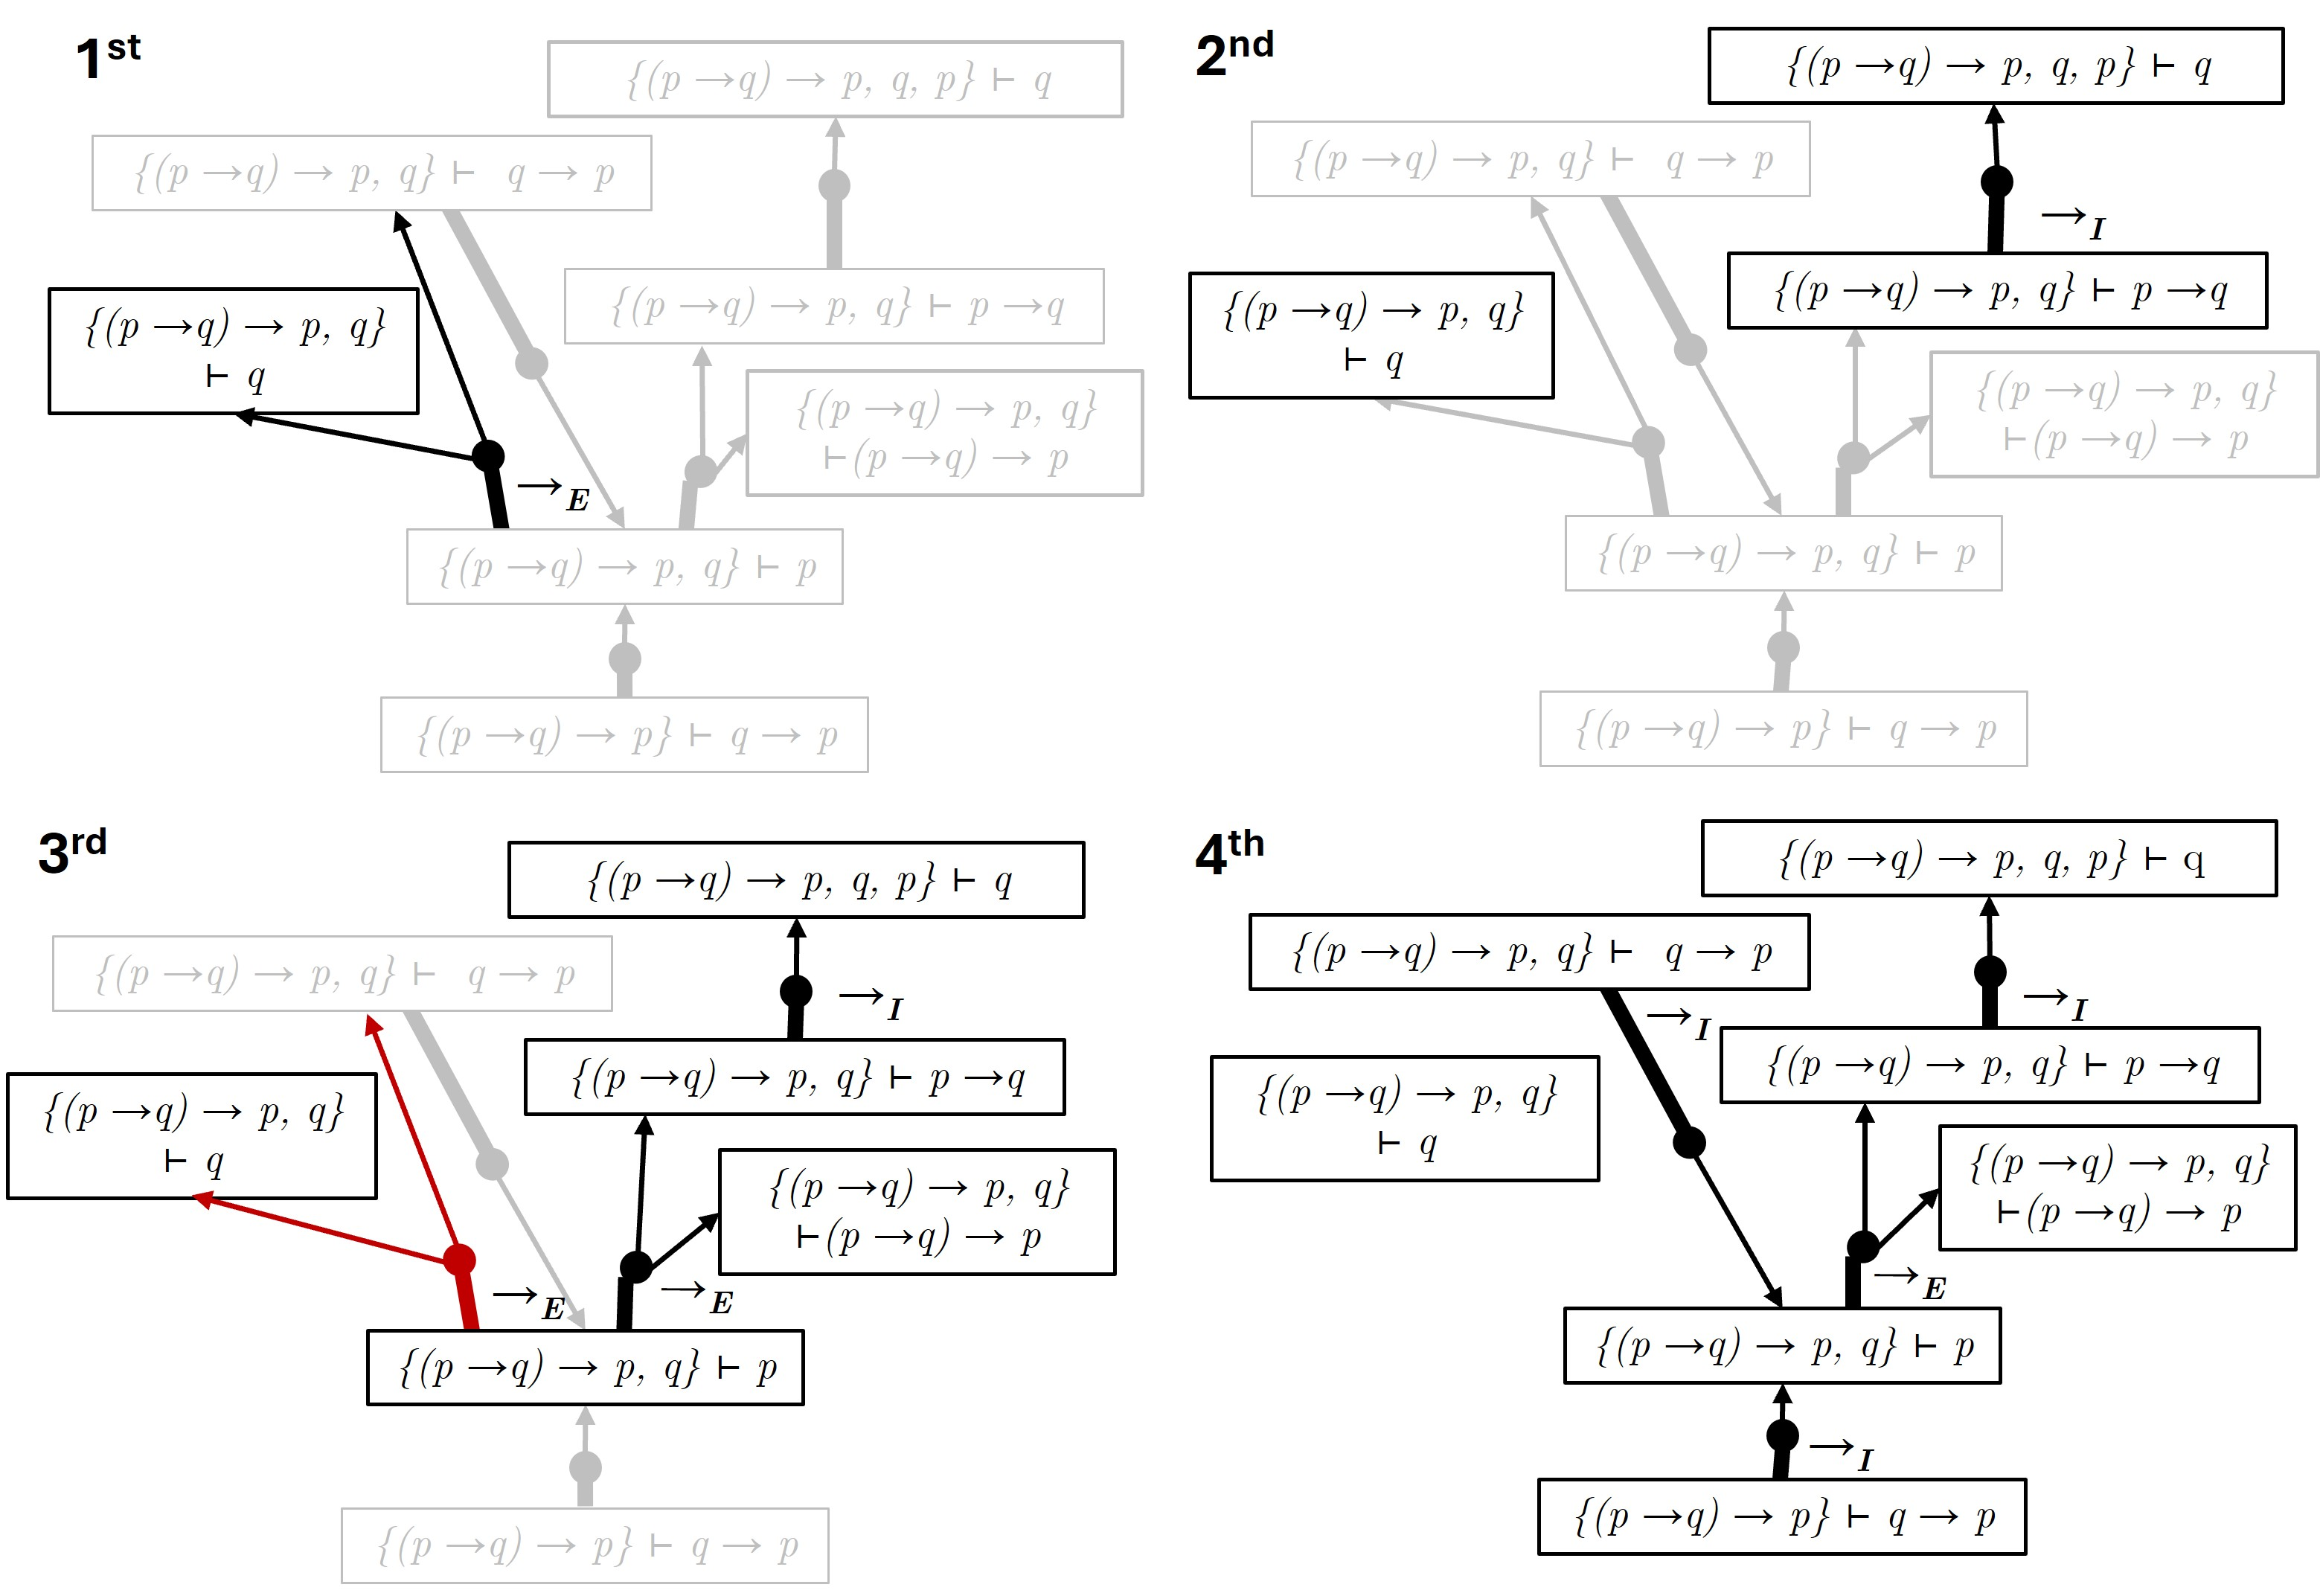
\includegraphics[width=1\linewidth]{Chapters/Figures/trim-gen.jpg}
    \caption{Step by step trimming process using the HTS on the PG presented in \autoref{fig:st-ex-final}. The last graph presents the final TPG of the entire process.}
    \label{fig:sg-trim-height}
\end{figure}

\subsubsection*{Size Trim Strategy} 
The \gls{STS} is similar to \gls{HTS}, but it tracks the size of each goal, defined as the number of formulas involved in a valid solution. Instead of retaining only the first edge, the algorithm explores all incoming edges and selects the one leading to the smallest proof, by using an adaptation of the \emph{uniform cost search} algorithm. This approach may cause a goal to be revisited multiple times, making it more computationally expensive. Nevertheless, it often produces more concise proofs in terms of the sequence of rule applications.

In this algorithm, we assign a number to each node to keep track of the minimum number of formulas required to prove it. The first step is to iterate over the leaves and assign the value~1 to them, since the shortest way to reach them is by using the formulas themselves. The subsequent iteration over the remaining nodes is shown in \autoref{fig:sg-trim-size} for the \gls{PG} presented in \autoref{fig:st-ex-final}.

\vspace{0.5em}
\textbf{Steps:}
\begin{enumerate}[align=left,labelwidth=*,labelsep=1em]
    \item[\textbf{\ordinalnum{1} and \ordinalnum{2}}] These first two steps are identical to the first two steps presented in \gls{HTS}, but in this algorithm a size value is assigned whenever a new node is added to the list of goals to be explored. This value is computed as the sum of the sizes of the head goals in an edge plus one (for the node itself).
    
    \item[\textbf{\ordinalnum{3}}] In this step, the algorithm explores the goal \(\{(p \to q) \to p, q\} \vdash (p \to q) \to p\), but no new nodes are added to be explored. It then explores the goal \(\{(p \to q) \to p, q\} \vdash p \to q\). This time, all heads of the incoming edge have already been explored, so the tail goal \(\{(p \to q) \to p, q\} \vdash p\) is added to be explored and assigned a size of 4, computed as 3 from the head nodes plus 1 for itself. Unlike \gls{HTS}, the algorithm does not discard the other outgoing edges, since their sizes have not been fully computed.
    
    \item[\textbf{\ordinalnum{4}}] At this stage, the goal \(\{(p \to q) \to p, q\} \vdash p\) is being explored. The goal \(\{(p \to q) \to p, q\} \vdash q \to p\) is added to the list of goals to be explored, since it has incoming edges, while \(\{(p \to q) \to p\} \vdash q \to p\) has none and is simply marked as explored. The sizes of these nodes are then computed.
    
    \item[\textbf{\ordinalnum{5}}] The goal \(\{(p \to q) \to p, q\} \vdash q \to p\) is explored. Its only incoming edge now has all heads explored, allowing the algorithm to check whether this path yields a smaller size than the one assigned to \(\{(p \to q) \to p, q\} \vdash p\). After computing the size considering this edge, the value is greater than the previously assigned size, so the edge is discarded.
    
    \item[\textbf{\ordinalnum{6}}] As there are no more goals to explore, the algorithm terminates. Each node now has a size value corresponding to the number of formulas required to reach a solution. This information is particularly useful, as it fulfills one of the objectives.
\end{enumerate}


\begin{figure}
    \centering
    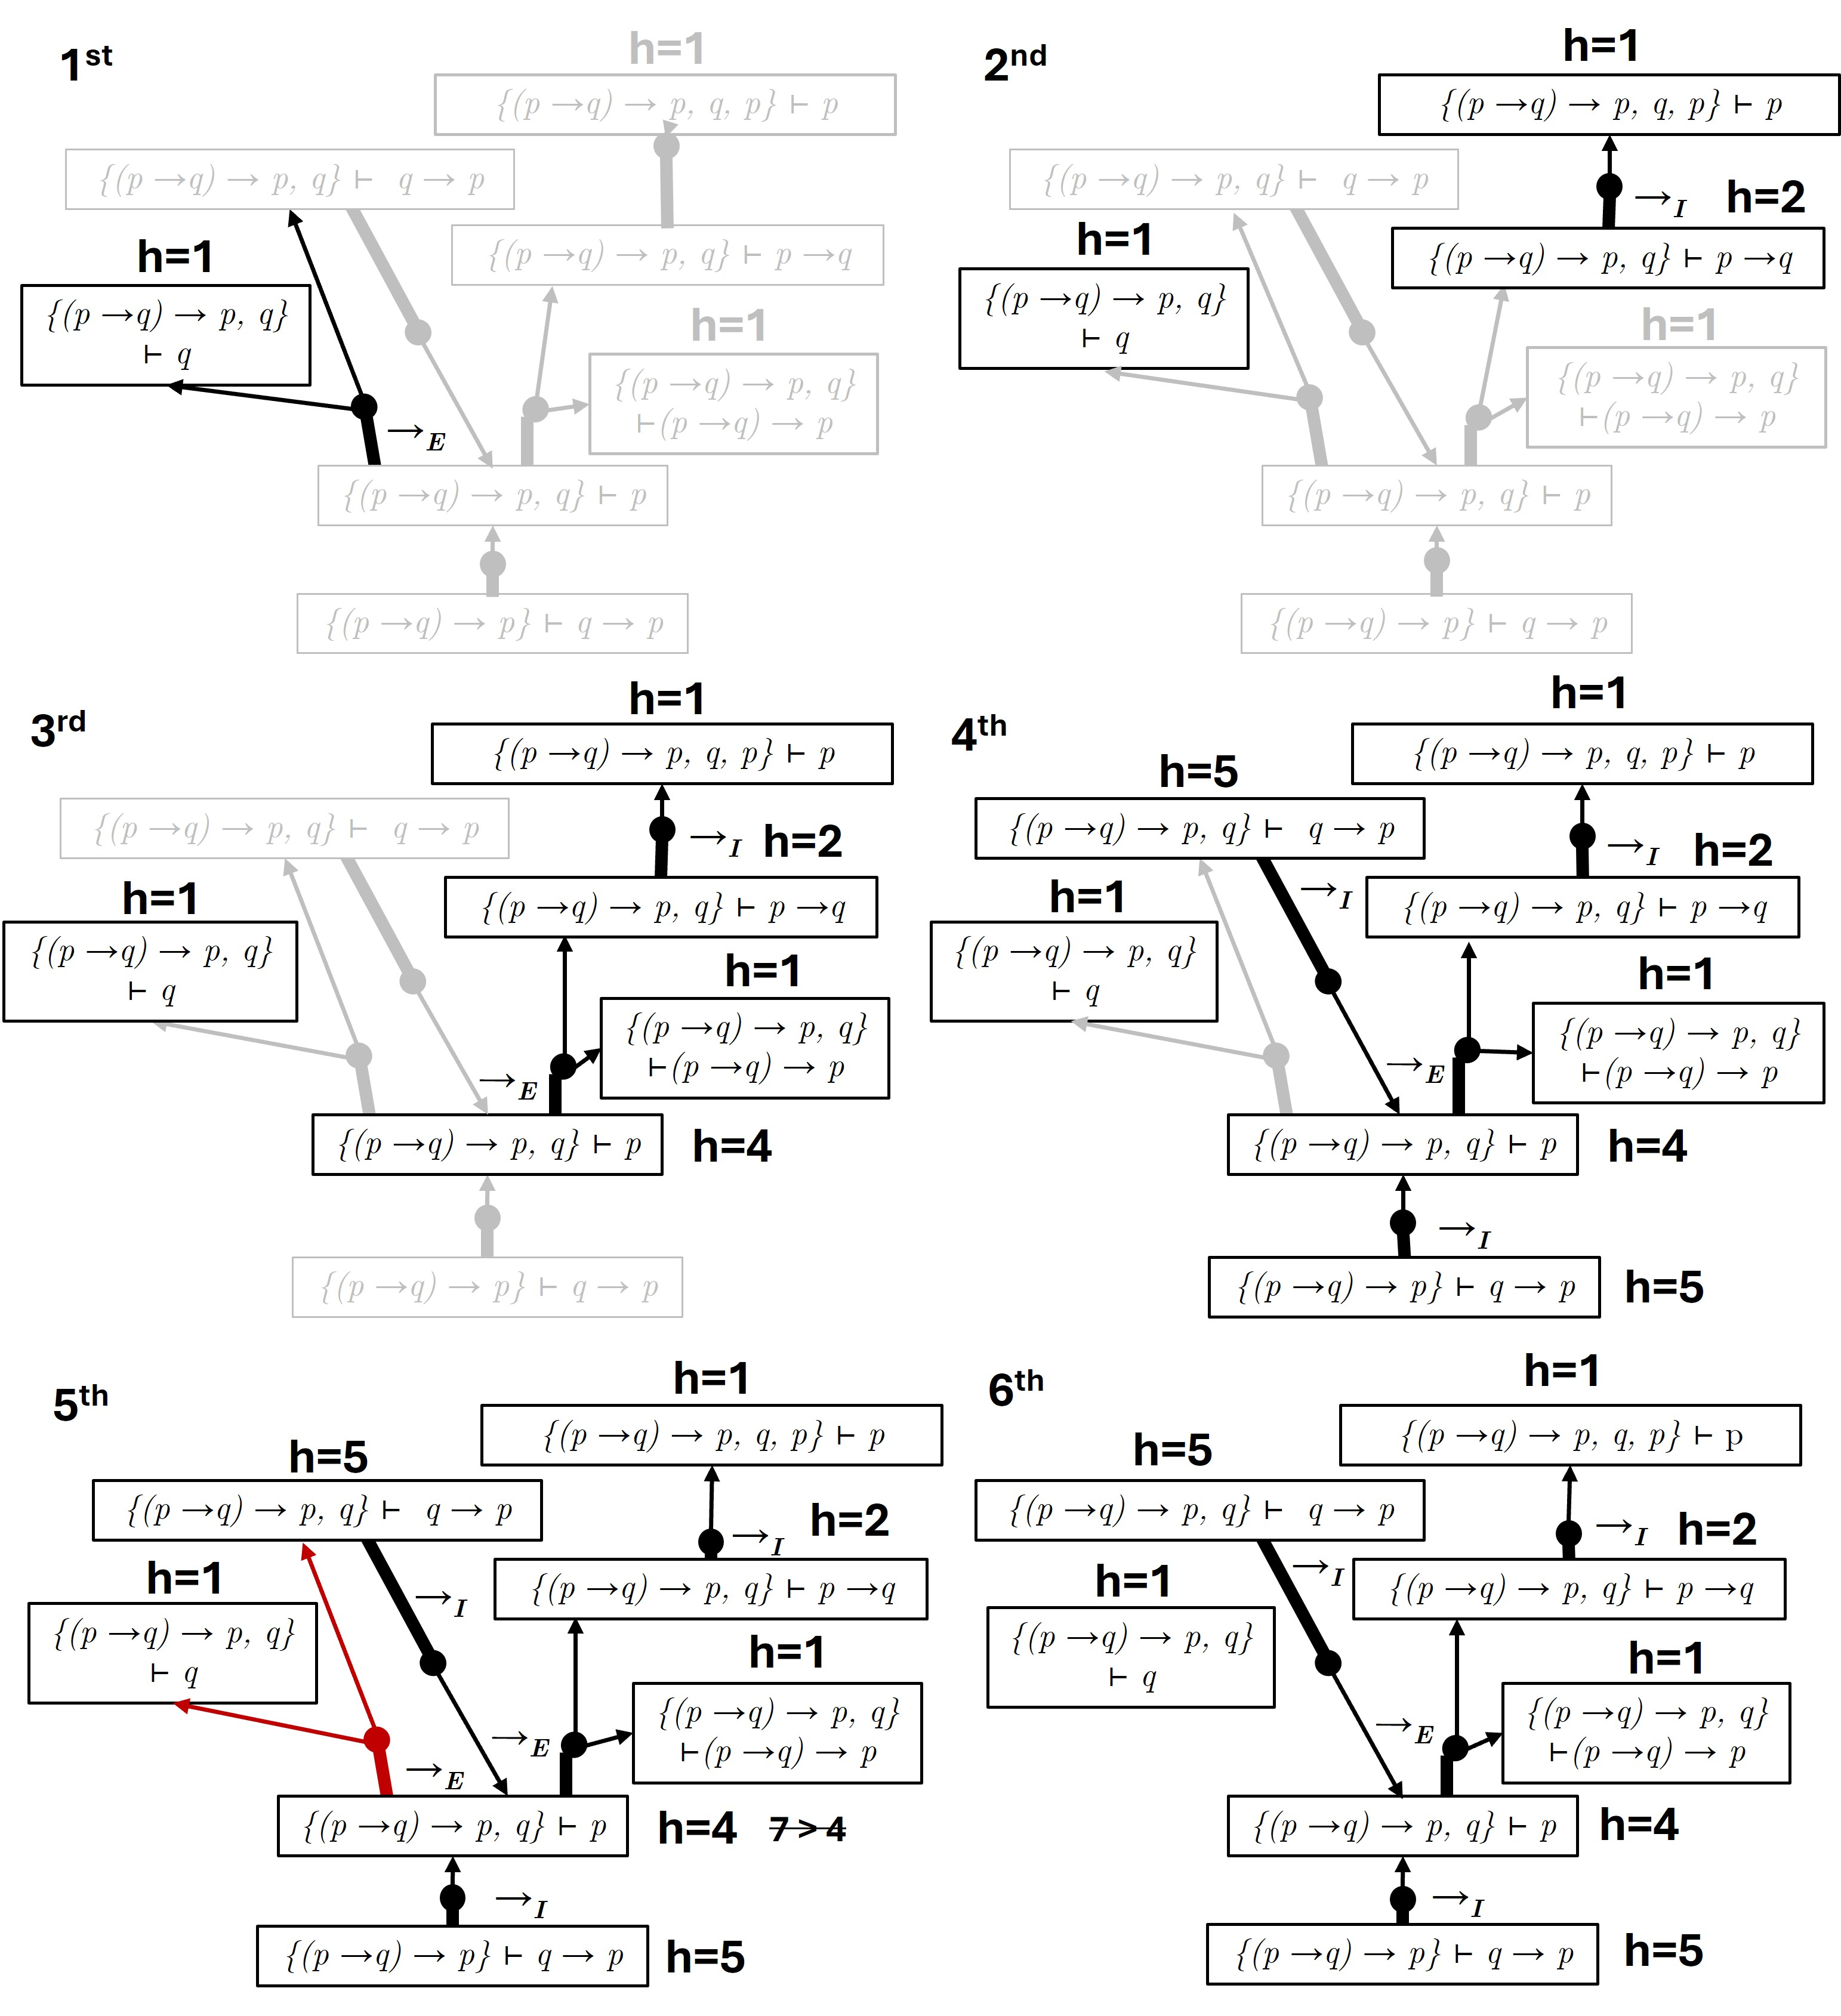
\includegraphics[width=1\linewidth]{Chapters/Figures/trim-2-gen.jpg}
    \caption{Step by step trimming process using the STS on the PG presented in \autoref{fig:st-ex-final}. The last graph presents the final trimmed graph of the entire process.}
    \label{fig:sg-trim-size}
\end{figure}

\vspace{1em}

The resulting trimmed graphs, in these examples, are the same but is not always the case. For example, for the problem \(\vdash a \lor \lnot a\) the output graph is different so the edges considered are different leading to different solutions. Using the \gls{HTS} the result best tree has height 6 and size 12 but in \gls{STS} the height is 7 and the size is 9. \autoref{fig:final-equivalent} and \autoref{fig:final-equivalent1} show the different optimal proofs for the two strategies. The reason for considering multiple strategies is that one of them may produce a proof closer to the human reasoning process. The choice of strategy depends on the problem itself. For example, in the previous problem (\(\vdash a \lor \lnot a\)), the \gls{STS} result is closer to human reasoning because of the order in which the rules are applied.

\begin{figure}[h!]
\centering
\small
\centering
\begin{prooftree}

  \AxiomC{${a}^2$}
  \RightLabel{$(\lor_{I_r})$}
  \UnaryInfC{$a \lor \lnot a$}

  \AxiomC{${\lnot(a \lor \lnot a)}^1$}

  \RightLabel{$(\lnot_E)$}
  \BinaryInfC{$\bot$}
  \RightLabel{$(\bot,2)$}
  \UnaryInfC{$\lnot a$}

  \AxiomC{${\lnot a}^3$}
  \RightLabel{$(\lor_{I_l})$}
  \UnaryInfC{$a \lor \lnot a$}

 \AxiomC{${\lnot(a \lor \lnot a)}^1$}

  \RightLabel{$(\lnot_E)$}
  \BinaryInfC{$\bot$}
  \RightLabel{$(\bot,3)$}
  \UnaryInfC{$\lnot \lnot a$}
    
  \RightLabel{$(\lnot_E)$}
  \BinaryInfC{$\bot$}
  \RightLabel{$(\bot, 1)$}
  \UnaryInfC{$a \lor \lnot a$}
\end{prooftree}

\caption{HTS result for the problem \(\vdash a \lor \lnot a\) has height 6 and size 12}
\label{fig:final-equivalent}
\end{figure}
\begin{figure}[h!]
\centering
\small
\centering
\begin{prooftree}

  \AxiomC{${a}^2$}
  \RightLabel{$(\lor_{I_r})$}
  \UnaryInfC{$a \lor \lnot a$}

  \AxiomC{${\lnot(a \lor \lnot a)}^1$}

  \RightLabel{$(\lnot_E)$}
  \BinaryInfC{$\bot$}
  \RightLabel{$(\bot,2)$}
  \UnaryInfC{$\lnot a$}
  \RightLabel{$(\lor_{I_l})$}
  \UnaryInfC{$a \lor \lnot a$}

 \AxiomC{${\lnot(a \lor \lnot a)}^1$}
    
  \RightLabel{$(\lnot_E)$}
  \BinaryInfC{$\bot$}
  \RightLabel{$(\bot, 1)$}
  \UnaryInfC{$a \lor \lnot a$}
\end{prooftree}

\caption{STS result for the problem \(\vdash a \lor \lnot a\) has height 7 and size 9.}
\label{fig:final-equivalent1}
\end{figure}

The final graph, shown in \autoref{fig:trimmed}, still contains all the solutions presented in \autoref{fig:sol-pg-pl}. None of them were lost, as all the proved goals were preserved. The idea of this graph is that it can be queried multiple times to generate feedback. 

\begin{figure}[H]
    \centering
    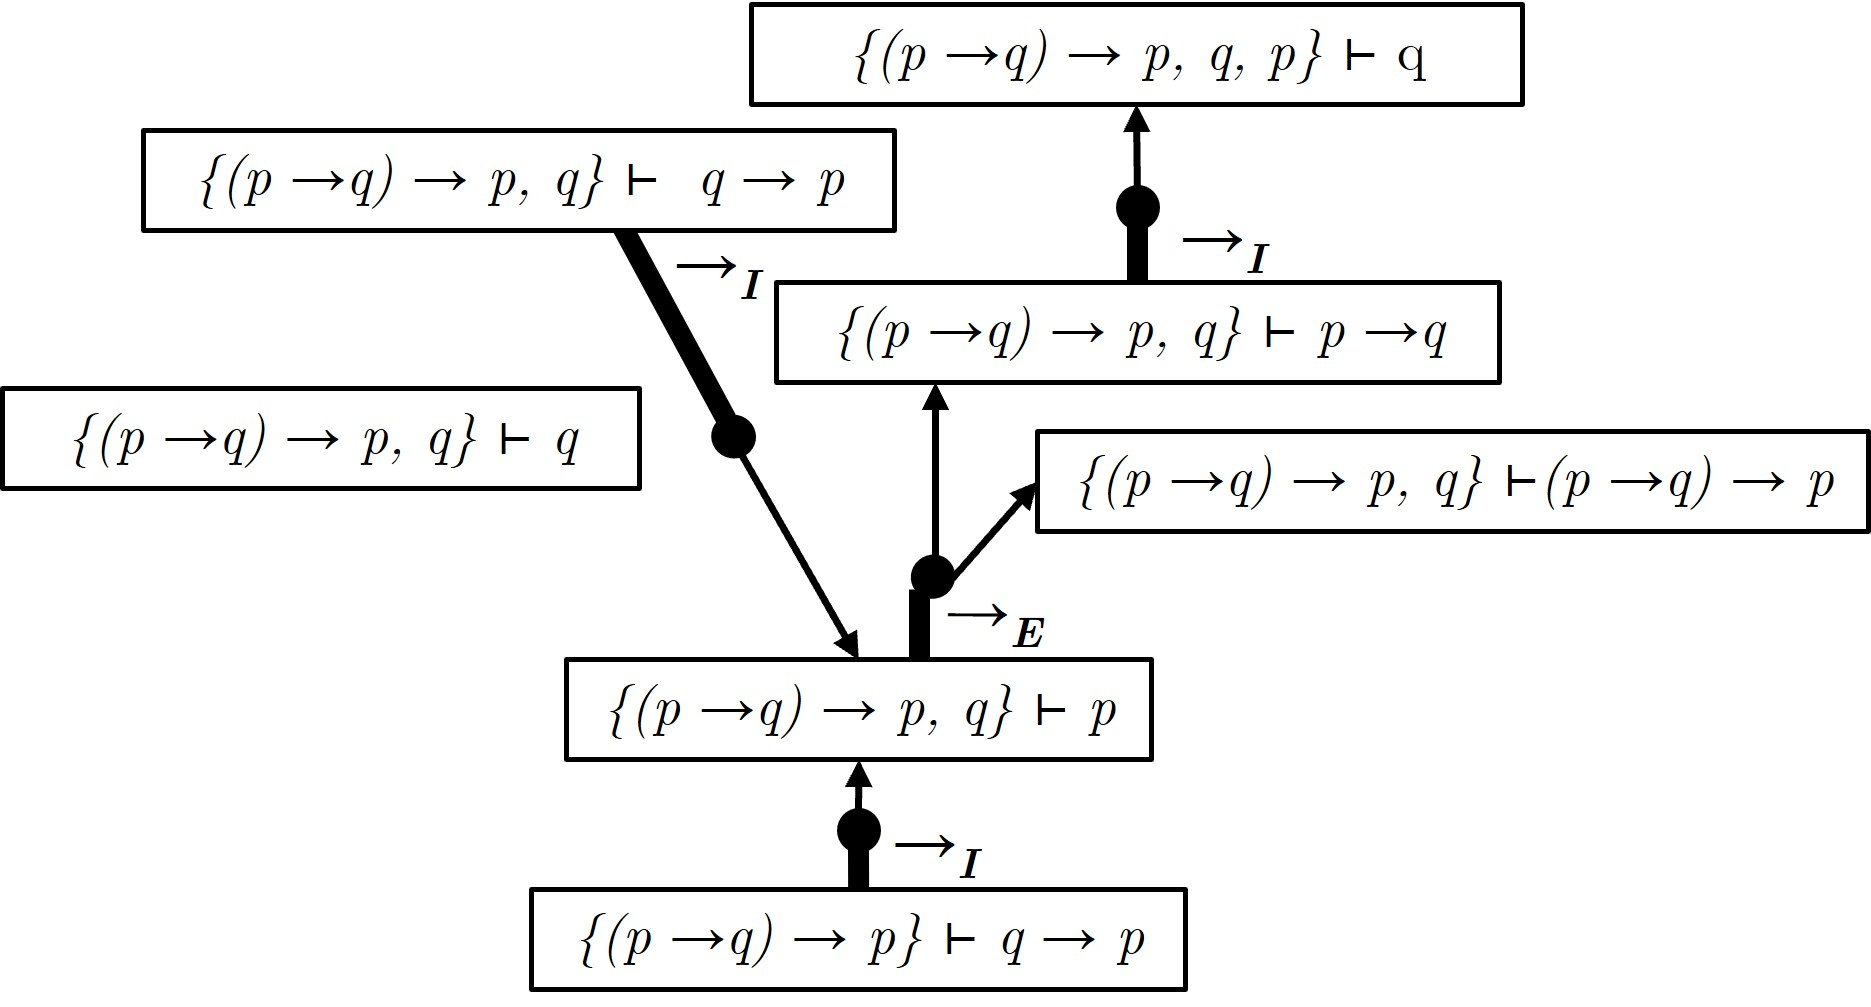
\includegraphics[width=0.7\linewidth]{Chapters/Figures/trimmed.jpg}
    \caption{Final trimmed graph on the PG presented in \autoref{fig:st-ex-final} for both strategies.}
    \label{fig:trimmed}
\end{figure}

To extract a solution from the \gls{TPG}, we first select a goal. If the goal is present in the graph, we traverse its nodes until there are no further nodes to explore. Since the graph has already been trimmed, we are guaranteed that the resulting solution is both valid and the shortest one available. During the traversal, the algorithm keeps track of the new assumptions introduced at each step. These assumptions are marked by comparing the difference between the previous goal and the next goal along a transition. For example, consider the transition from \(\{(p \to q) \to p, q\} \vdash p \to q\) to \(\{(p \to q) \to p, q, p\} \vdash p\) In this case, the new assumption is \(p\), and the algorithm assigns a new mark to it. 

%A final complete solution for the goal \(\{(p \to q) \to p, q\} \vdash p\) is shown in \autoref{fig:sol-extract}, extracted from the final graph in \autoref{fig:trimmed}.

%\begin{figure}[H]
%\centering
%\begin{prooftree}
%  \AxiomC{$\overset{1}{q}$}
%  \RightLabel{$(\to_I, 1)$}
%  \UnaryInfC{$p \to q$}
  
%  \AxiomC{$(p \to q) \to p$}
  
%  \RightLabel{$(\to_E)$}
%  \BinaryInfC{$p$}
%\end{prooftree}
%\caption{Extracted solution for the goal \(\{(p \to q) \to p, q\} \vdash p\) using the final graph from \autoref{fig:trimmed}}
%\label{fig:sol-extract}
%\end{figure}

\section{Feedback Generation}
With the final graph, and a way to extract solutions given a target goal as input we can now generate feedback by querying which goals remain unproved in the student's proof. How can we guarantee that our algorithm satisfies all the objectives previously established? Let us cover the objectives one by one the and give examples on how we can use the algorithm:

\subsection*{Context-aware feedback}
 This is achieved in two different ways, when constructing the graphs by consider multiple solutions and keeping all of them instead of storing the best one found. This way, even if the student shifts from, what would be the optimal solution, the algorithm can still find solutions to their problem. The other way is by considering the state of the proof when the student introduces new formulas. For example, if the user shifts from the track of the graph of the algorithm, when we query the algorithm it cannot find a solution because the formula that we are looking does not belong to the \gls{TG}, different when the formula belongs but there is no goal in the \gls{PG}. In this cases by running the algorithm again including the new formulas as input we will eventually, find a solution for that specific problem. This way, our algorithm is not restricted to guiding users to a fixed solution, instead, it can guide them to the solution that best fits the student's reasoning.

\autoref{fig:fed-1} illustrates the first approach, where the student chose a different path from the optional solution by applying the \(\to_E\) rule with \(q\) and \(q \to p\), which corresponds to the rule that was removed during the trimming process (the red edge). By querying the graph in \autoref{fig:trimmed} with the remaining goal to be proven, we can still extract a valid solution.

\begin{figure}[ht]
\centering
\small
\begin{minipage}{0.44\linewidth}
\centering
\textbf{Incomplete proof}
\begin{prooftree}
  \AxiomC{${q}^1$}
  \noLine
  \AxiomC{$\textbf{\large ?}$}
  \UnaryInfC{$q \to p$}
  
  \RightLabel{$(\to_E)$}
  \BinaryInfC{$p$}
  \RightLabel{$(\to_I, 1)$}
  \UnaryInfC{$q \to p$}
\end{prooftree}
\end{minipage}%
\hfill
\begin{minipage}{0.01\linewidth}
\centering
\rule{0.4pt}{3cm} % vertical line: width x height
\end{minipage}%
\hfill
\begin{minipage}{0.52\linewidth}
\centering
\textbf{Proof found}\\
Target goal: \(\{(p \to q) \to p, q\} \vdash q \to p\)
\begin{prooftree}

  \AxiomC{${q}^2$}
  \RightLabel{$(\to_I)$}
  \UnaryInfC{$p \to q$}
  
  \AxiomC{$(p \to q) \to p$}
  
  \RightLabel{$(\to_E)$}
  \BinaryInfC{$p$}
  \RightLabel{$(\to_I, 2)$}
  \UnaryInfC{$q \to p$}

\end{prooftree}
\end{minipage}
\caption{Extracting a non-optimal solution using the TPG shown in \autoref{fig:trimmed}.}
\label{fig:fed-1}
\end{figure}

\autoref{fig:fed-2} illustrates the second approach, where the student introduces new formulas that were not considered during the decomposition phase. By running the algorithm considering the new formula \(p \land q\), it can find a solution for the new problem.

\begin{figure}[ht]
\centering
\small
\begin{minipage}{0.38\linewidth}
\centering
\textbf{Incomplete proof}
\begin{prooftree}

  \AxiomC{$\textbf{\large ?}$}
  \noLine
  \UnaryInfC{$p \land q$}

  \AxiomC{${p \land q}^2$}
  \RightLabel{$(\land_{E_r})$}
  \UnaryInfC{$p$}
  \RightLabel{$(\to_I, 2)$}
  \UnaryInfC{$(p \land q) \to p$}

  \RightLabel{$(\to_E)$}
  \BinaryInfC{$p$}
  
  \RightLabel{$(\to_I, 1)$}
  \UnaryInfC{$q \to p$}
\end{prooftree}
\end{minipage}%
\hfill
\begin{minipage}{0.01\linewidth}
\centering
\rule{0.4pt}{3cm} % vertical line: width x height
\end{minipage}%
\hfill
\begin{minipage}{0.58\linewidth}
\centering
\textbf{Proof found}\\
Target goal: \(\{(p \to q) \to p, q\} \vdash p \land q\)
\begin{prooftree}

  \AxiomC{${q}^1$}
  \RightLabel{$(\to_I)$}
  \UnaryInfC{$p \to q$}
  
  \AxiomC{$(p \to q) \to p$}
  
  \RightLabel{$(\to_E)$}
  \BinaryInfC{$p$}
  
  \AxiomC{${q}^1$}
  
  \RightLabel{$(\land_I)$}
  \BinaryInfC{$p \land q$}

\end{prooftree}
\end{minipage}
\caption{Extracting a solution from a different TPG considering \(p \land q\).}
\label{fig:fed-2}
\end{figure}

\subsection*{Providing guidance on rule applications} This can be achieved by exploring the trimmed graph and identifying the target goal. If the goal is present in the graph, the applicable rule can be determined by examining the outgoing edges. For example, for the goal \(\{(p \to q) \to p, q\} \vdash p\) and the \gls{TPG} presented in \autoref{fig:trimmed}, we can suggest applying the Elimination of the Introduction rule, since its application guarantees that the user will reach a solution.

\subsection*{Breaking proofs into smaller sub-proofs} Similarly to the previous objective, we can provide a sub-goal as feedback instead of a rule. By identifying the target goal, we can extract any ancestor goal to present as feedback. This methodology is meaningful only for problems of some complexity, particularly in cases where certain steps are not obvious, such as problems that require reasoning by contradiction.

\subsection*{Indicating the distance to a solution} This objective is straightforward. We simply need to determine the number of rules traversed from the target goal to the leaves of the graph. For example, in the scenario presented in \autoref{fig:fed-1}, by examining either the solution or the graph, we can see that the user is three rule applications away from a solution, specifically from the optimal solution identified by the algorithm starting from our target goal.

\subsection*{Improvements in the proof:} We can suggest improvements to the student's solution by comparing it with the optimal solution identified by the algorithm. If the student's solution is more complex, involving more rules or formulas than the optimal one, we can compare the two solutions side by side to identify the point of divergence. From that step, we can prompt the user to explore alternative ways to reach a solution.

\section{Implementation}
The main focus during the implementation was to develop a system that is extensible, readable, maintainable, and easy to use. To implement the algorithm, we used the Java programming language \cite{java}, as the rest of the project was also in Java and it is easier to integrate with existing components. To achieve this, we applied two well-known design patterns: the \emph{Strategy} pattern and the \emph{Builder} pattern. We decided to split the algorithm into two main components: one responsible for producing the \gls{TG}, and the other responsible for building the \gls{PG} (see \autoref{fig:graphs-overview}).

\begin{figure}[h]
    \centering
    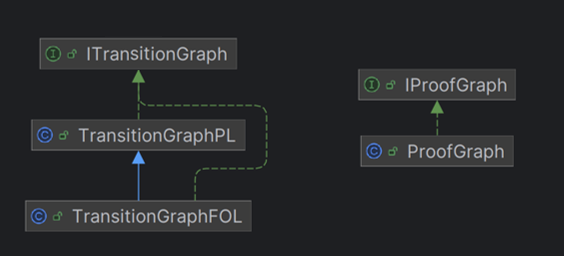
\includegraphics[width=0.5\linewidth]{Chapters/Figures/graphs.png}
    \caption{Overview of the two main components: Transition Graph and Proof Graph.}
    \label{fig:graphs-overview}
\end{figure}

For the \gls{TG}, we implemented the algorithms previously presented. The underlying graph structure is identical to the formal definition, therefore we created two classes: \texttt{TransitionGraphNode} (representing labeled heads) and \texttt{TransitionGraphEdge} (representing hyperedges). These classes encapsulate all possible rule applications that can occur in a proof, providing a direct mapping between the formal definition of the graph and its implementation.

For the \gls{PG}, we adopted the \emph{Strategy} pattern. The construction process requires a builder strategy (the algorithm that creates the proof graph) and a trimming strategy (the algorithm that filters goals to keep only the relevant ones). The use of the \emph{Strategy} pattern is crucial here, since it allows us to extend the system by introducing new builders or trimming strategies without modifying the existing code. For instance, we could create a builder strategy that applies parallelization techniques to improve efficiency, and plug it into the system without breaking existing functionality. This flexibility was achieved by defining a \emph{Build Strategy} and a \emph{Trim Strategy} interface.

\begin{figure}[h]
    \centering
    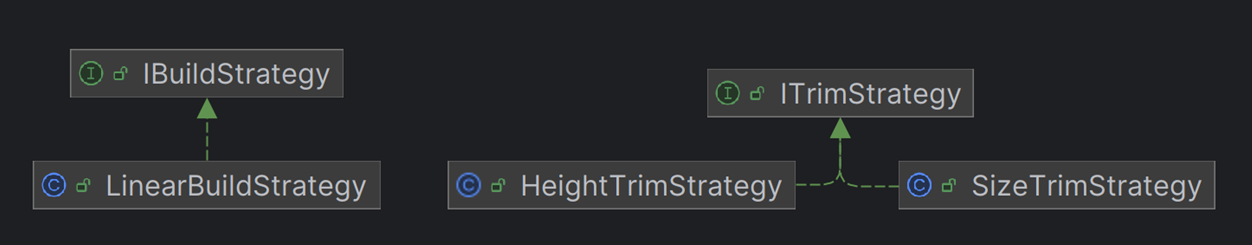
\includegraphics[width=0.8\linewidth]{Chapters/Figures/strategies.png}
    \caption{\emph{Build Strategy} and a \emph{Trim Strategy} implementation overview.}
    \label{fig:strategies}
\end{figure}

In the \texttt{LinearBuildStrategy} class we implemented the algorithm described in \autoref{alg:pg-construction}, including adaptations for \gls{FOL}. Once again, the proof graph is implemented in direct correspondence with its formal definition in \autoref{def:pg}: we defined a \texttt{ProofEdge} class and a \texttt{GoalNode} class with the same characteristics.
For trimming, we implemented two strategies: the \texttt{HeightTrimStrategy} class (which implements the \gls{HTS} algorithm) and the \texttt{SizeTrimStrategy} class (which implements the \gls{STS} algorithm).
To assemble the final proof, we created a \texttt{Solution} class. This class receives the \gls{TPG} and a target goal as arguments, and attempts to construct the proof by traversing the graph. 
Since proof graphs grow rapidly (as discussed in previous sections), and since different problems may require different configurations of the algorithm, we introduced the \texttt{ProofSettings} class. This class centralizes all customizable parameters of the algorithm (see \autoref{fig:proof-settings}).

\begin{figure}
    \centering
    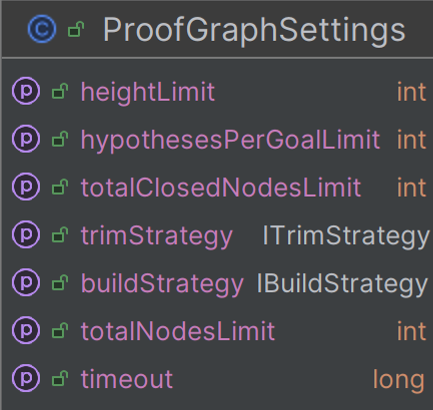
\includegraphics[width=0.3\linewidth]{Chapters/Figures/settings.png}
    \caption{The \texttt{ProofSettings} class stores customizable parameters of the algorithm.}
    \label{fig:proof-settings}
\end{figure}

We defined five different stopping conditions:
\begin{itemize}
    \item \textbf{heightLimit}: Limits the height of the final proof. This avoids generating overly complex solutions. For example, if we know that the optimal solution has a certain height and the current user solution has a different height, we compute the difference and add a small threshold, such as two or three steps. The algorithm will then only search for solutions within this height interval.
    \item \textbf{hypothesesPerGoalLimit}: Limits the number of hypotheses per goal. This prevents generating solutions where the user introduces excessive assumptions compared to the expected solution.
    \item \textbf{totalClosedNodesLimit}: Limits the number of closed nodes (leaves) in the \gls{PG}, thereby constraining the number of solutions stored.
    \item \textbf{totalNodesLimit}: Similar to the previous condition, but applied to the total number of nodes explored during \gls{PG} construction.
    \item \textbf{timeout}: Limits the execution time for generating the \gls{PG}. This is essential to ensure responsiveness and to prevent long waiting times.
\end{itemize}

To create an instance of the algorithm, several components must be specified. To simplify this process and improve readability, we adopted the \emph{Builder} pattern. The code in \autoref{lst:code-algo-instance} shows a real example of how an instance is created for a \gls{FOL} problem with different configurations.

\begin{lstlisting}[style=javastyle,
  caption={Example of an instantiation of the algorithm for a First-Order Logic problem with multiple configurations.},
  label={lst:code-algo-instance}]
            Solution solution = new @@AlgoProofFOLBuilder@@(
                // Define the main goal
                new @@AlgoProofFOLMainGoalBuilder@@(conclusion)
                    .addPremises(premises)
                    // Add auxiliary variable
                    .addTerm(new @@ASTVariable@@("a")))       
            .addForbiddenRule(@@ERule@@.ABSURDITY)
            .se\gls{TG}oal(
                // Define the target goal
                new @@AlgoProofFOLGoalBuilder@@(conclusion)
                    .addHypothesis(hypotheses))
            .setAlgoSettingsBuilder(
                // Define settings
                new @@AlgoSettingsBuilder@@()
                    .setHypothesesPerState(5)
                    .setTimeout(1500)
                    .setHypothesesPerGoal(Integer.MAX_VALUE)
                    .setTrimStrategy(new @@SizeTrimStrategy@@()))
            .build();
\end{lstlisting}

Default settings are provided, so it is not necessary to specify every parameter in each instance. For example, since there is currently only one build strategy, it does not need to be explicitly set. Once instantiated, the \texttt{Solution} object can be used to query the algorithm multiple times, generate solutions for problems, and provide feedback to users.

In summary, the implementation was designed to be both extensible and maintainable. By separating the construction of the \gls{TG} and the \gls{PG}, and by introducing modular components, and customizable proof settings, we ensured that the system can easily adapt to new requirements and extensions. This flexible design not only supports efficient proof generation but also provides a solid foundation for experimenting with different strategies and configurations, which is essential for the practical application of the algorithm in an interactive environment.

\subsection{Tests} 
During the implementation, the IntelliJ profiler was used to monitor both memory usage and execution time. This allowed us to identify potential bottlenecks and optimize the algorithm to ensure efficient performance.

To ensure the correctness of the algorithm, its output was compared against a set of exercises referenced in \autoref{nd-exercises}, verifying that the solutions produced matched the expected results. Additionally, unit tests were conducted to simultaneously evaluate both the ND proof interpreter, as described in [REF], and the algorithm itself, ensuring that the generated proof graphs satisfy the expected logical properties and that the system behaves consistently across different scenarios.

\subsection{Performance}
A key feature of our algorithm that distinguishes it from other approaches is that we do not keep only a single solution, but rather a set of possible solutions. This design avoids recomputing the entire algorithm when generating feedback for the same problem. Since the algorithm is integrated with an interactive online tool, responsiveness is essential: users expect immediate feedback and cannot afford long waiting times. 

A good example where storing multiple solutions instead of only one is beneficial can be found in practical classes, where the interactive tool can act as support. Imagine a teacher asking students to solve a set of exercises. In this scenario, the feedback requested by students will often be very similar. By keeping a trimmed graph with multiple solutions, the system reduces the number of feedback misses, and in most cases the algorithm needs to be computed only once per problem. Furthermore, when a student requests feedback once, they usually request additional feedback for the same problem. Having multiple solutions precomputed directly improves efficiency in such cases.

Nevertheless, this strategy comes at a cost in terms of space, as the system must store thousands of goals. A promising future improvement would be to maintain a database with precomputed trimmed graphs for the most common queries. This would reduce memory usage by storing them externally and applying the algorithm only in less frequent cases where the student diverges from the direct solution. Another strategy involves implementing heuristics designed to prioritize proofs that align more closely with human reasoning. When all possible proofs are considered during the construction of the \gls{PG}, some steps may still be regarded as unnecessary, since they can lead to a solution but do so in an overly complex manner, even when appropriate stopping conditions are applied.

When applied to \gls{FOL} problems, the algorithm faces additional challenges. \gls{FOL} is more expressive than \gls{PL} and introduces extra components that affect performance. The most significant factor is the number of terms in a problem, together with the auxiliary ones required to prove it. For problems with many terms, the resulting \gls{TG} and consequently the \gls{PG} can become very large. By examining the number of loops in \autoref{alg:transitions-1}, the reason for this growth becomes clear. In addition, three inference rules particularly affect performance: Elimination of the Disjunction (\(\vee_E\)), Elimination of the Negation (\(\lnot_E\)), and Elimination of the Existential (\(\exists_E\)). All of them introduce multiple hypotheses, which leads to wider \gls{PG}s.

These limitations only become problematic when dealing with very complex problems. Since this project is developed for pedagogical purposes, the problems encountered by the system will generally be simpler and more direct. \autoref{nd-exercises} presents a list of some of the exercises used both to test the algorithm and to conduct the performance evaluation.

The experiments were executed on a computer with an Intel(R) Core(TM) i7-8750H CPU @ 2.20GHz (2.21GHz) and 32GB of RAM. The histograms in \autoref{fig:histogram-time-formulas-pl} and \autoref{fig:histogram-time-formulas-fol} illustrate the computation times, where the x-axis represents time in milliseconds and the y-axis represents the number of problems. These results correspond to the computation of full solutions for the problems in \autoref{nd-exercises}, including the generation of the three graphs using \gls{STS}. A clear contrast can be observed: in \gls{PL}, most problems (\(75\%\)) are solved within 50 milliseconds, while in \gls{FOL}, that generaly are more complex exercises the same proportion requires about 500 milliseconds. Overall, these values are very good for the system we developed. In practice, user waiting times are often shorter, since we can reuse the graphs already generated to produce feedback. Thus, only problems that introduce new formulas not considered during the decomposition step need to be recomputed.


\begin{figure}[h]
    \centering
    \begin{minipage}{0.49\textwidth}
        \centering
        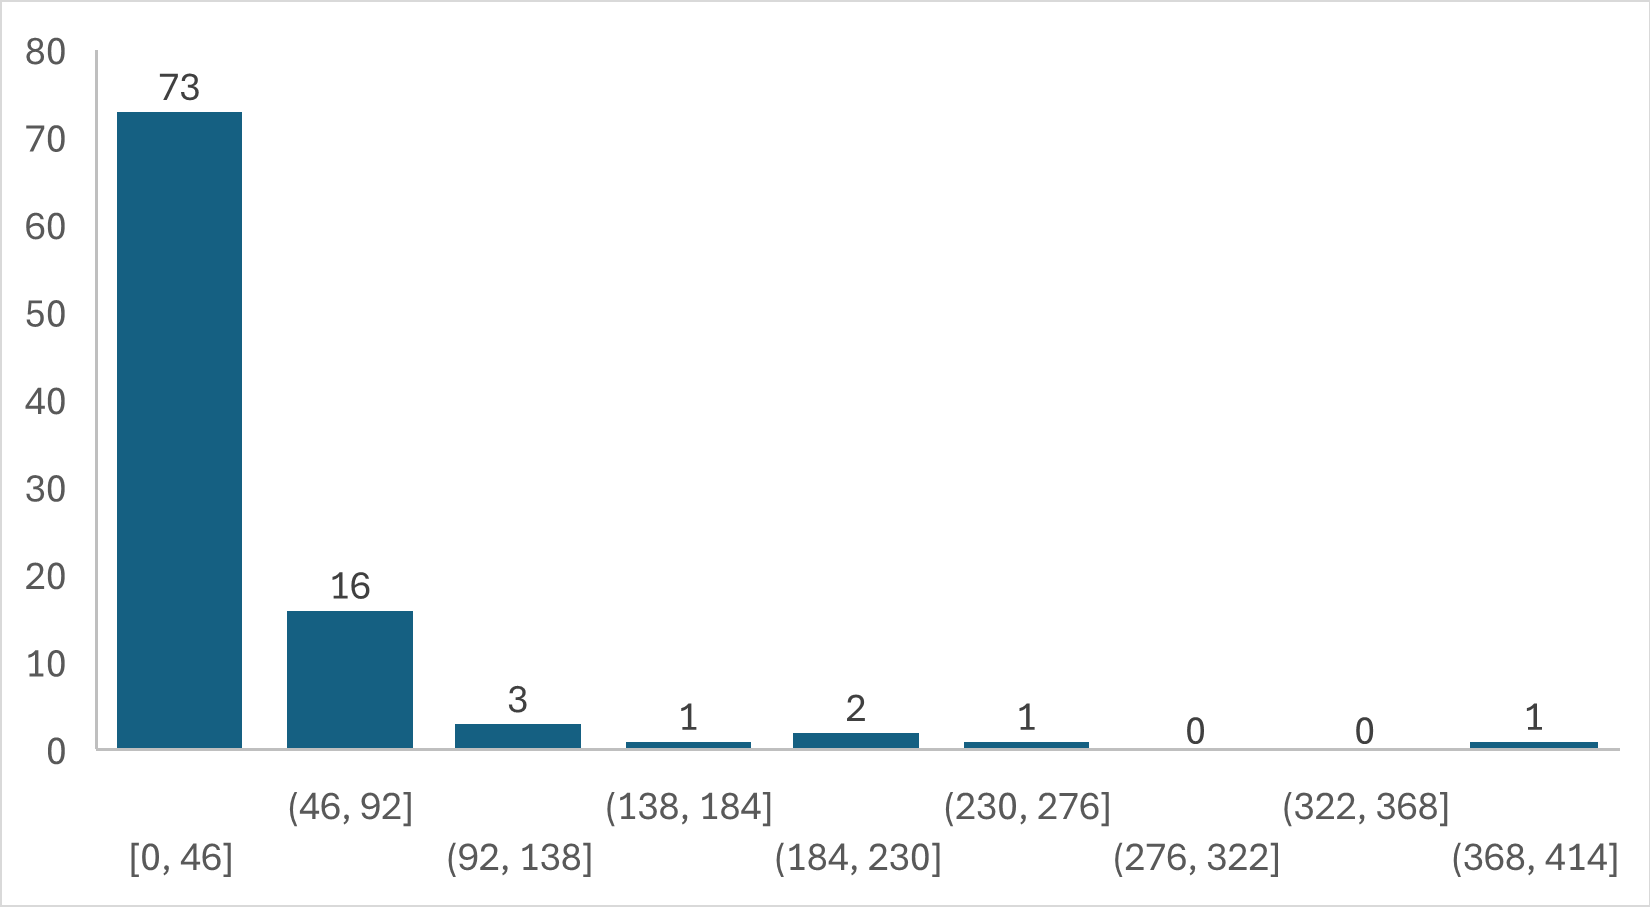
\includegraphics[width=\linewidth]{Chapters/Figures/time_formulas_histogram_pl.png}
        \caption{Histogram of time per problem using PL problems}
        \label{fig:histogram-time-formulas-pl}
    \end{minipage}
    \hfill
    \begin{minipage}{0.49\textwidth}
        \centering
        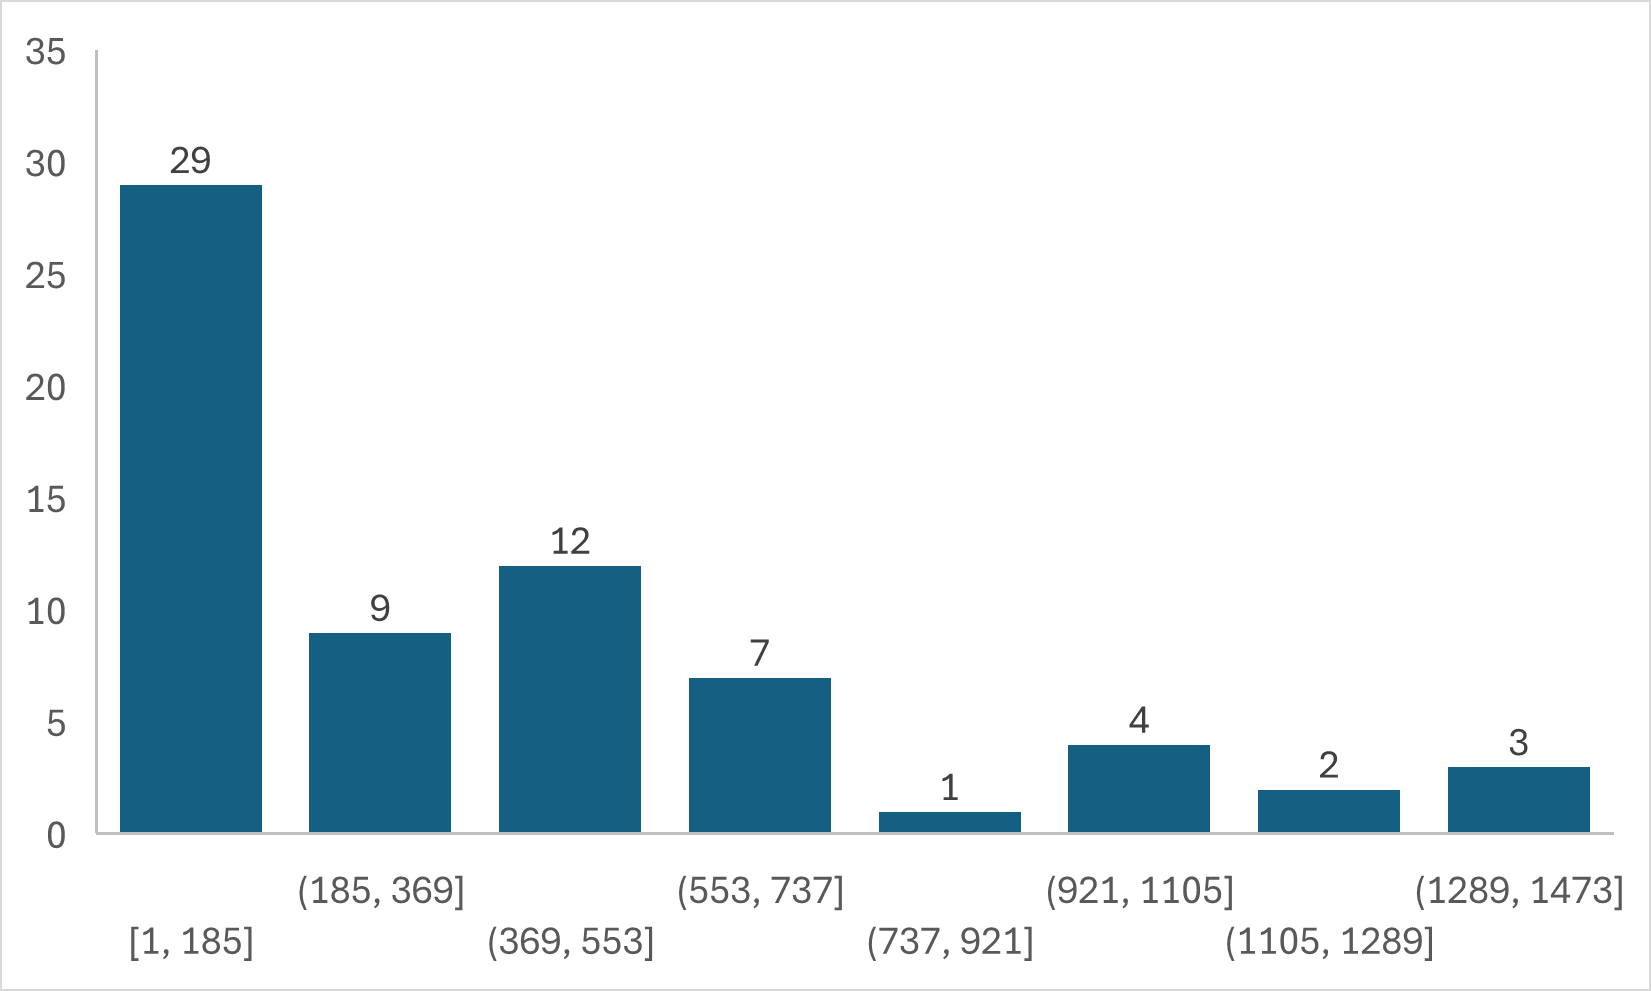
\includegraphics[width=\linewidth]{Chapters/Figures/time_formulas_histogram_fol.png}
        \caption{Histogram of time per problem using FOL problems}
        \label{fig:histogram-time-formulas-fol}
    \end{minipage}
\end{figure}

Another experiment examined the relation between the number of formulas (corresponding to the formulas in the decomposition step) and the computation time. As shown in \autoref{fig:formulas-time-pl} and \autoref{fig:formulas-time-fol}, the time generally increases with the number of formulas. This effect is especially pronounced in \gls{PL}, where the larger number of terms leads to significantly more formulas.

\begin{figure}[h]
    \centering
    \begin{minipage}{0.48\textwidth}
        \centering
        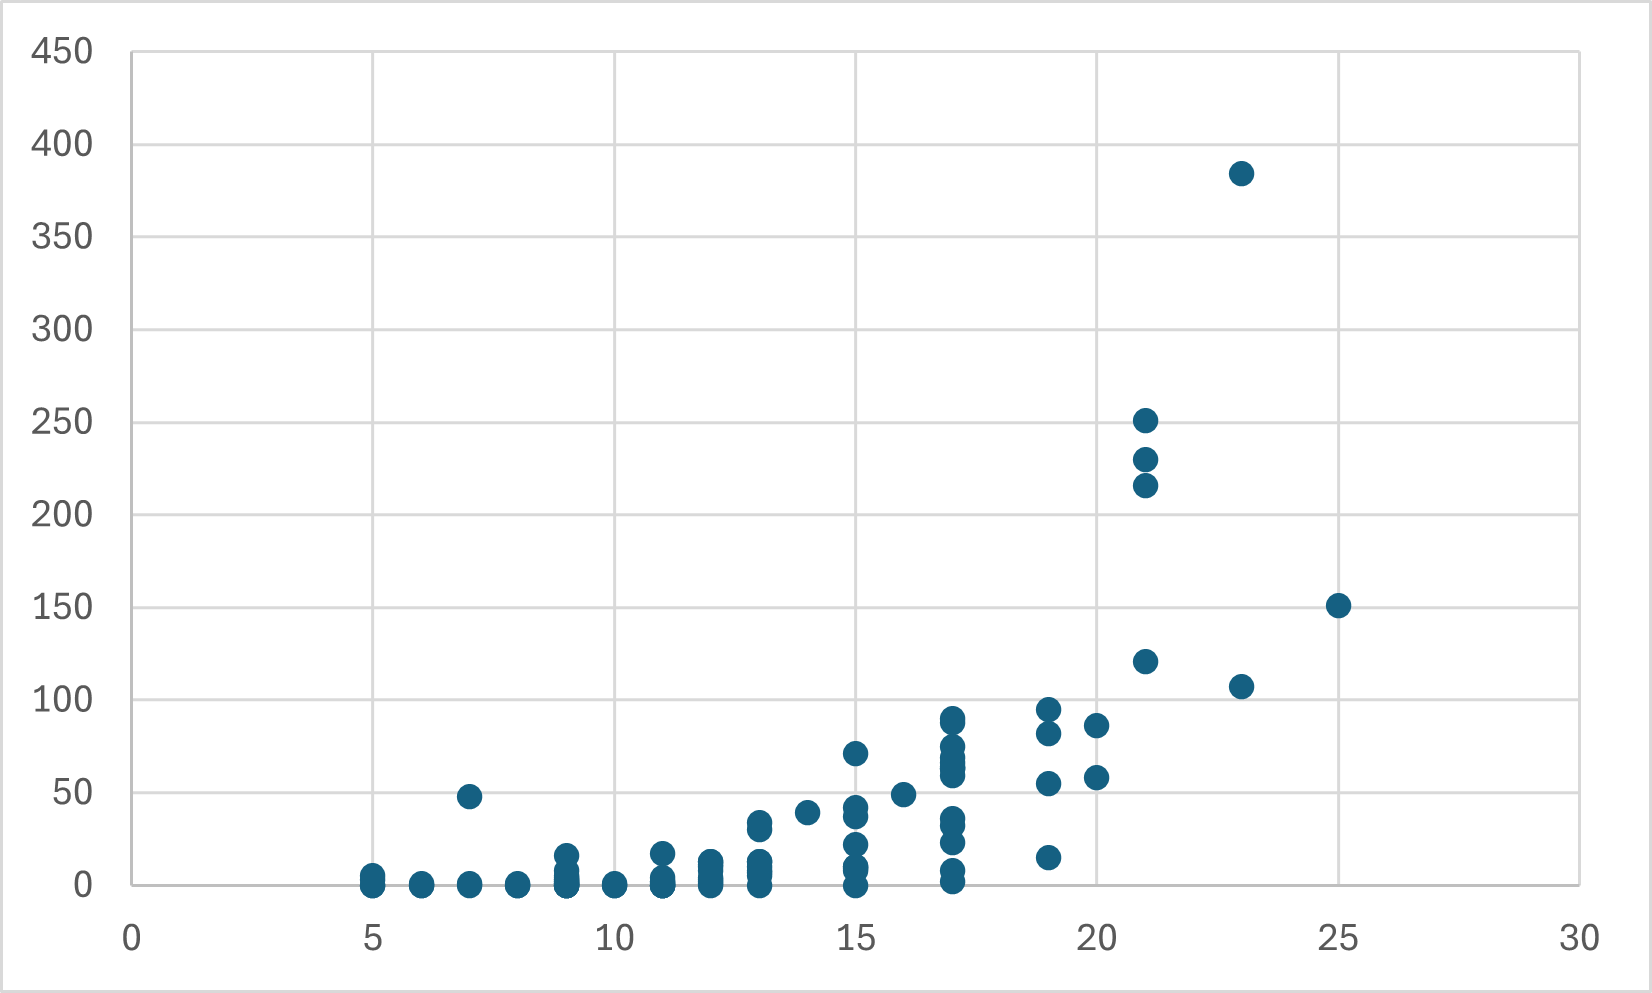
\includegraphics[width=\linewidth]{Chapters/Figures/time_formulas_pl.png}
        \caption{Scatter plot of formulas versus time using PL problems}
        \label{fig:formulas-time-pl}
    \end{minipage}
    \hfill
    \begin{minipage}{0.48\textwidth}
        \centering
        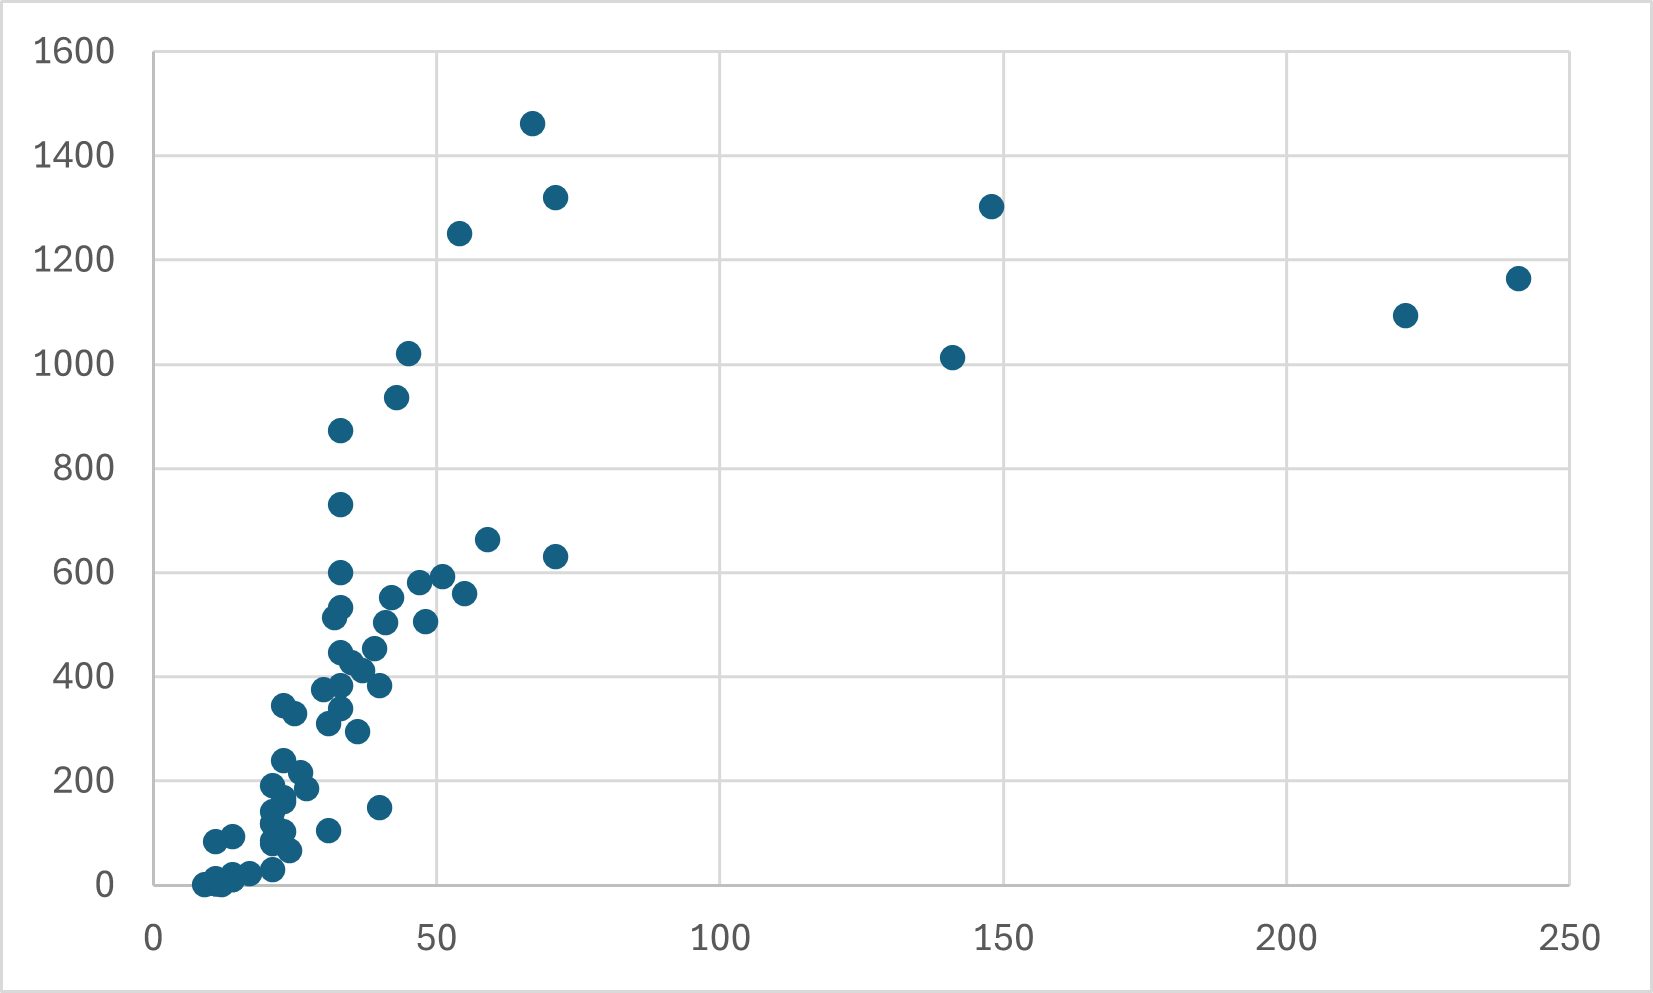
\includegraphics[width=\linewidth]{Chapters/Figures/time_formulas_fol.png}
        \caption{Scatter plot of formulas versus time using FOL problems}
        \label{fig:formulas-time-fol}
    \end{minipage}
\end{figure}

In conclusion, it is crucial to define appropriate stopping conditions for each problem in order to achieve better performance, since no universal configuration can solve every problem efficiently. Moreover, the effectiveness of these stopping conditions may also depend on the machine where the algorithm is executed.

\section{Future work}
The algorithm presented in this work has been implemented and, as shown in the previous section, it provides very good results for pedagogical exercises. However, there are several aspects that can be improved. One challenge is handling large graphs and keeping them in memory. An alternative approach, already mentioned, is to maintain a database with precomputed trimmed graphs for the most common queries. In this way, we only need to retrieve the solution from the database and do not need to load the full graph.

The algorithm can also be applied in assignments to evaluate proofs. By comparing the student's solution with the one found by the algorithm, we can measure how far the student's solution is from a possible solution. This allows us to assess the quality of the resolution and provide a grade accordingly.

Another possible application is the generation of new problems. If we run the algorithm without the trimming step, we can produce multiple sub-problems from an initial problem. From the resulting graph, we can extract several problems and even select them according to their difficulty, based on factors such as the rules applied, the number of formulas and rules, and the number of hypotheses generated.
